\documentclass[11pt]{book}
\usepackage[labelfont={bf}, margin=1cm]{caption}
\usepackage{titling, titlepic}
\usepackage{multirow}
\usepackage[colorinlistoftodos, bordercolor=white, backgroundcolor=cyan]{todonotes}
\usepackage{booktabs, caption, subcaption}
\usepackage{hyperref, comment}
\usepackage{algpseudocode, algorithm}
\begin{document}

\begin{center}

\vspace{2.5cm}

% [CHANGE] The title of your thesis. If your thesis has a subtitle, then this
% should appear right below the main title, in a smaller font.
\begin{Huge}
Deadline Driven Behavior in Intelligent Virtual Environments
\end{Huge}
\todo[inline]{Plaatje}
\vspace{1.5cm}

% [CHANGE] Your full name. In case of multiple names, you can include their
% initials as well, e.g. "Jan G.J. van der Wegge".
Djura S. Smits
% [CHANGE] Your student ID, as this has been assigned to you by the UvA
% administration.
5619807

\vspace{1.5cm}

% [DO NOT CHANGE]
Master's thesis\\
% [CHANGE] Whether your Bachelor thesis is 6 ECTS (regular) or 9 ECTS (Honours
% programme).
Credits: 48 EC

\vspace{0.5cm}

% [DO NOT CHANGE] The name of the educational programme.
Master's in Artificial Intelligence

\vspace{0.25cm}

% [DO NOT CHANGE] The addess of the educational programme.
University of Amsterdam\\
Faculty of Science\\
Science Park 904\\
1098 XH Amsterdam

\vspace{4cm}

\emph{Supervisor}\\
% [CHANGE] The name of your supervisor. Include the titles of your supervisor,
% as well as the initials for *all* of his/her first names.
Arnoud Visser\\
Philip Kerbush

\vspace{0.25cm}

% [CHANGE] The address of the institute at which your supervisor is working.
% Be sure to include (1) institute (is appropriate), (2) faculty (if
% appropriate), (3) organisation name, (4) organisation address (2 lines).
Intelligent Systems Lab\\
Faculty of Science\\
University of Amsterdam\\
Science Park 904\\
1098 XH  Amsterdam

\vspace{1.5cm}

% [CHANGE] The date at which you will finalize and submit your thesis.
\todo{Change}
June 24th, 2010

\end{center}
\newpage

%\documentclass[11pt]{book}

%\title{Deadline Driven Behavior in Intelligent Virtual Environments}
%\author{ Djura Smits}
%\date{\today}
%\titlepic{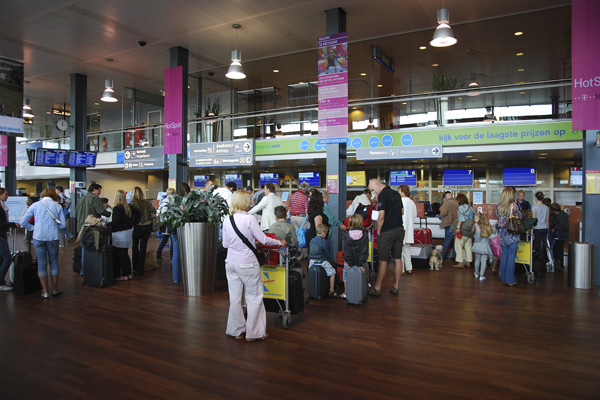
\includegraphics[width=\textwidth]{rotterdamairportphoto.jpg}}



\graphicspath{{.}{../results}}

%\begin{document}
\listoftodos
\newpage
%\maketitle
 %\chapter*{\centering Abstract}
%\addcontentsline{toc}{chapter}{Abstract}
%\abstract
%\maketitle
%\newpage
 %\chapter*{\centering Acknowledgements}
%\addcontentsline{toc}{chapter}{Abstract}
%\maketitle
%\abstract
%\newpage
\section{Acknowledgements}
I would like to thank my supervisors Philip Kerbush from TNO, and Arnoud Visser from the UvA. Furthermore, I would like to thank Ernst Bovenkamp for providing the data and videos from Rotterdam airport. I would also like to thank my friends and family for the support, and my classmates, many of whom I've enjoyed working with for many years.
\newpage
\tableofcontents
\newpage

\chapter{Introduction}
%\todo[inline]{introduction}
%\todo{How to place pedestrian simulation in the whole spectrum of AI related studies?}
Artificial intelligence is the branch of computer science that aims to create or simulate intelligence in machines. The range of methods to attempt this is endless. One of the many subfields in AI is aimed at reproducing human behavior. The problem of recreating human behavior can be tackled from many different perspectives. For example, one could attempt to get an understanding of the workings of the human mind, and try to imitate this in a computer program. Another approach would be to treat the human brain as a black box, and mainly focus on recreating external behavior. In this approach it does not matter whether the inner workings of this computer program are simular to that of an actual human being. The disadvantage of this approach is that it does not help you learn how the human mind works. However, when used for practical purposes, approaching the problem like this is favorable, since it is more likely to run real-time and take up less resources. In our research, we are attempting to recreate a specific kind of human behavior. Namely, the kind of behavior that one would encounter in a public environment.\\
\begin{figure}[h]
\begin{center}
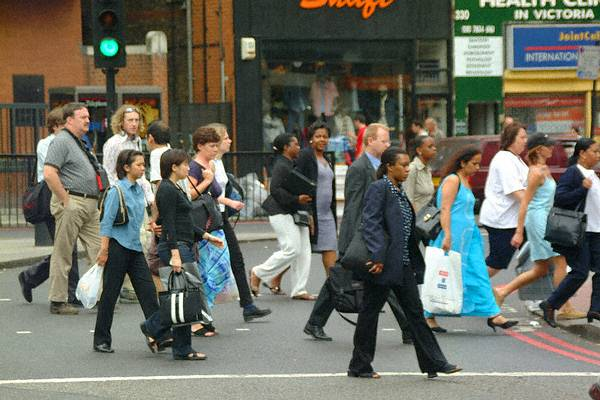
\includegraphics[width=200pt]{pedestrians.jpg}
\label{pedestrianpicture}
\end{center}
\caption{People going about their everyday business}
\end{figure}
For the last decade or so, there has been an increased interest in reinforcing security in public environments. The recent advances in technology have increased the feasibility of many different methods. An important approach in this area of interest is the automatic detection of suspicious behavior from camera images. The approaches in this area can vary, but one important aspect that they have in common, is the necessity of camera footage to be able to test the approaches. Since it can be extremely tedious to collect and annotate this data it would be very rewarding to be able to generate testing data on the fly. It is beyond the scope of our research to get into what suspicious behavior looks like, so we like to focus on the behavior of "non-suspicious" people. Assuming that so-called "normal" people greatly outnumber terrorists, these suspicious people could be added in later with ease. In other words, we would like to be able to quickly generate crowds of people doing normal, everyday behavior.\\
Simulation of pedestrians is a widely studied subject. Many models have been created for the various characteristics that arise when multiple human-like agents move around in the same area. Many uses can be thought of for pedestrian simulation. An important purpose for this could be for example to easily create a large amount of "normal" pedestrians (as opposed to "suspicious" pedestrians).  Suspicious pedestrians whose behavior is scripted by hand can then be placed in the environment to easily create artificial testing data for suspicious behavior detection algorithms and the like. Furthermore, the addition of simulated virtual pedestrians can add realism to otherwise mostly empty battlefield scenarios.\\
Another way to look at the behavior of groups of pedestrians is to explicitly specify how they behave when they enter a certain type of situation. In our approach, we would like to be able to specify behavior by drawing situations on an environment. For example, when a food stand is present in the area, we would like to be able to indicate that the agents that are placed in the neighborhood of that stand are able to do certain food-buying behavior.

An additional requirement is that we would like to indicate a certain \emph{deadline} for an agent which is the time at which its goal is not reachable any more. This approach results in roughly two types of behavior, \emph{hurried} and \emph{relaxed}. When the deadline approaches, less and less actions are likely to be done, since actions that take much time would result in not reaching the goal in time.\\
We validated our model by mimicking certain behaviors found on Rotterdam airport. We chose Rotterdam airport because time restrictions are very prevalent in a departure hall like the one on Rotterdam airport.

So, to summarize, we would like to create a system that enables a user to easily place large amounts of more or less realistically behaving people in an environment. These people should behave in a way appropriate for the environment. Furthermore, the behavior should be guided by the fact that every pedestrian has a fixed deadline for when he has to do his final activity. Ideally, this will lead to a distinction between hurried and relaxed behavior, depending on whether the deadline is near or still far away. In order to facilitate defining the behavior, we will create a tool to easily design these behaviors as Petri-nets. Petri-nets are a mathematical modelling language mainly used for describing distributed processes. In this thesis we will show that they are also suitable for modelling human behavior, especially when it involves interactions with multiple people.
\todo[inline]{Describe the promise for the utopia of my research}


%In many fields using simulation, the environments are empty except for the absolutely necessary parts of the simulation. However, the environment would look much more realistic if actual civilians would walk around. That is why SIMOBS was developed. SIMOBS is a plugin for the VR-Forces simulation application that makes it easy to quickly generate residential areas inhabited by families, and factories where these civilians go to work. However, at the moment these virtual pedestrians only walk from their houses to their work and back at fixed points in time. The purpose of this thesis is to extend this SIMOBS plugin to create more realistic behavior.

\section{SIMOBS}
SIMOBS is a plugin for the military simulation toolkit VR-forces (\url{http://www.mak.com/products/vrforces.php} It is a tool for generating and executing battlefield scenarios. SIMOBS is a plugin developed to quickly generate inhabitants of an area by drawing residential areas and plants on the map in VR-forces. The behavior of these inhabitants is determined by \emph{Daily Motion Patterns}, which specify where certain types of inhabitants need to go at specified times. This is the idea that forms the basis for our research.


%\todo[inline]{Tweak research question.}
\section{Research Question}
The question we are going to base this research around is the following:
\begin{quote}
How can an intelligent virtual environment for simulated pedestrians be extended to deal with time-restricted destinations?
\end{quote}
Some of these terms may need some clarification:
\begin{itemize}
%\item \emph{Distributed}:\\
 %We are using a distributed environment to simulate our pedestrians. This means that various tasks such as path planning can be delegated to other services and are not of our concern. Therefore, we can afford to focus more on higher level behavior.
\item \emph{Intelligent Virtual Environment}:\\
IVE is a broad term, but in this particular case we mean that a large portion of the intelligence needed for the pedestrians to walk around is placed in the environment, instead of in the pedestrians walking in it. There are different ways to construct an IVE, which is something we have to look at as well.

\item \emph{Time-restricted destinations}:\\
We would like to create a framework that is able to deal with departure hall-like situations. That means that pedestrians will have a destination (e.g. a train, or an airplane, etc.) that will be available for a limited amount of time (until it departs). It can also be used to create simulations with a pattern that is more realistic when run for a long period of time (such as a whole day). Furthermore, in many situations, only the time is known when the person has to arrive at his destination. In those cases it is more intuitive to define the time of arrival, instead of determining at what time someone has to leave his starting point. In the rest of the article, we will refer to these time restrictions as \emph{deadlines}.
\end{itemize}

We are going to solve this question by trying to answer the following subquestions:
\begin{itemize}
\item \emph{To what extent can pedestrians be simulated realisticly?}\\
If it were feasible to model the complete human brain, we would probably get the most lifelike behavior. However, since this is not possible, we have to simplify the model somehow. Models can be made in varying levels of complexity. Most often, a higher complexity means slower performance. That is why we have to think about getting the right balance between realism and performance. We also have to decide how we define realism. Do we take the inner model into account, or do we purely compare the resulting behavior to real people in similar situations?

\item \emph{How do we let the pedestrians make decisions based on time left to reach the destination?}\\
In situations such as departure halls, people have a destination (e.g. airplane, train) that is only available for a limited amount of time. Some actions might take a very short amount of time, some may need more. How do we let these pedestrians decide between the different options?

\item \emph{Is it possible to have emergent behavior based on time restrictions?}\\
Ideally, our model should lead to behavior that we have not expressly implemented in our system. In the context of time restrictions, we would like the pedestrians to have hurried or relaxed behavior based on the amount of time they have left to reach their goal.

%\item \emph{What kind of freedoms/restrictions do distributed systems give us?}\\
%As a consequence of using a distributed system we can delegate certain tasks to other units. On the other hand, our model also %needs to be compatible with the other units in the distributed system.

\item \emph{Is it possible to quickly generate these virtual pedestrians without much tweaking for each environment?}
\\We aim at creating pedestrians that can be used in many different environments without much additional scripting. Is it possible to do this and still have varied behavior between environments?
%\item How can the simulation be efficient without sacrificing too much realism?

\end{itemize}

%How do we create an \emph{intelligent virtual environment} framework so that \emph{realistic}, real-time acting virtual pedestrians can be generated \emph{quickly}, working with VR-forces and \emph{daily motion patterns}?
%\end{quote}
%Some terms will need some clarification about how we interpret them:
%\begin{itemize}
%\item \emph{Intelligent Virtual Environment}\\
%In an intelligent virtual environment, objects contain the rules about interacting with them, instead of the pedestrians.
%\item \emph{Realistic}:\\
%Crowds should move in a somewhat realistic manner and interact with the environment. Individuals should follow a logical path, making seemingly logical choices about what objects to interact with. Realistic refers to how the pedestrians act, not to their decision making model.
%\item \emph{Quick}:\\
%Requires as little specification as possible. Same specification for pedestrians have to be appropriate in many different environments.
%\item \emph{Daily Motion Patterns}:\\
%Things about the framework can be changed, but it may be preferrable to leave the Daily Motion Patterns in. DMPs require that pedestrians go to certain locations at certain times of the day.
%\end{itemize}

%This main question leads to a range of subquestions.
%\begin{quote}
%How do we balance realism and performance?
%\end{quote}
%How many pedestrians do we want to move around at the same time? How far does this limit the complexity of the models we can use?
%\begin{quote}
%How do we handle the planning?
%\end{quote}
%Daily motion patterns require the virtual pedestrians to be at a certain location at a certain time. How do we let the pedestrian decide for instance whether to go buy food or go to its train because it is almost leaving? Do we need to implement a model to handle basic needs such as hunger, and sleep, or will the pedestrians be able to act convincingly in another way?
%\begin{quote}
%What kinds of limits does the VR-forces framework give us?
%\end{quote}
%Our virtual pedestrians have to walk around in the VR-forces environment. This information has to be communicated to VR-forces in a certain way. This might restrict the possibilities of the simulation.


\chapter{Related Work}
% Tried to add tuples, but if I try to describe any more approaches with tuples, it would be like comparing apples and oranges.
%\todo[inline]{Indicate tuples for every approach (as much as is possible).}
When studying existing methods for modeling pedestrian behavior, the amount of available literature is quite overwhelming. This is not surprising as a large part of AI research focuses on the imitation of human behavior. However, not all means of simulating pedestrian behavior are developed for the same purpose. What we would like to have in our system, is a method to design behavior in an environment in the same way that other objects in the environment are designed. That is, it should be possible to spatially place the behaviors in the environment. However, this does not limit our search much since it only divides our desired result into two layers; namely the overall structure of different behaviors placed in the environment, and the definition of these different behaviors. When we approach the subject as \emph{designing behavior in an environment}, the search becomes much more narrow and directed.

\section{Designing the Situation-Dependent Behaviors}
In our research, we can divide the subject of "behavior" in two layers.  First of all, we have the layer in which individual behaviors are described. However, this information is embedded in a framework that describes how these individual behaviors vary spatially. Let us start with focussing on these individual behaviors. This field knows many approaches. First of all, the focus can lie on the group as a whole. The different members of the group are then often viewed as particles that influence the other group members near them with attracting and repulsive forces. Other approaches view crowds as a group of individuals, and the members are given some kind of simplified psychological model. The motivation behind this simplified model is that this will lead to complex behavior when many of these simple units are put together in a large crowd. This effect is known as \emph{emergence}.\\

\section{Group Interaction}
The research of interaction in groups started with Reynolds' boids \cite{Reynolds87flocks} , where members of the group were seen as particles that exert both repulsive and attracting forces on the other members of the flock, depending on the distance to one another, and forces inwards from the outer contour of the flock, in order to remain in a certain shape.  This behavior is driven by three simple rules, namely \emph{separation} (avoiding crowding local flockmates), \emph{cohesion} (move toward center of mass of local flockmates), and \emph{alignment} (steering towards average heading of local flockmates). However, this flocking behavior is more suitable for modelling behavior of animals such as fish, and will not give a very plausible result when it is used to model humans. Because humans usually act in a way more complicated than a flock. However, many researches have built upon this idea of modelling large groups by viewing the members as particles.

\subsection{Global approaches}
Many models that have been proposed focus on crowds in panic situations. An example of a model for panic situations is the one proposed by Pelechano et al. \cite{citeulike1080090} who divided people in three categories: \emph{trained leaders}, who have complete knowledge about the building, \emph{untrained leaders}, who handle stress well, help others and will explore the building, and \emph{untrained non-leaders}, who might panic. \todo[inline]{Maybe sections have to be named differently, or previous reference has to be moved, the approach uses global effects, but also more individual models} Another example of simulating panic situations, can be found in the article of Helbing, Farkas, and Vicsek \cite{citeulike1656038}. In their model, people exert a repulsive interaction force to stay away from each other, an additional \emph{body force} slowing to counteract body compression, and a \emph{sliding friction force} when a pedestrian comes in contact with another pedestrian or the wall. This model can lead to several effects known to occur in real panic situations.\\
While these methods give a good insight into the movements in those particular panic situations, they are less suitable for experiments running over a longer period of time. Only in those few moments of panic, or when crowds are very dense, do these models represent a crowd realistically. What we are looking for, is a framework that gives realistic behavior over longer periods of time. Pelechano, Allbeck and Badler \cite{Pelechano:2007:CIA:1272690.1272705} have simulated high-density crowds for normal situations. They base the movement of the crowds on a simple wayfinding algorithm and a number of different psychological (impatience, panic, personality attributes, etc.) and physiological traits(e.g.locomotion and energy level). Furthermore, the agent is given perception and will react to objects and other pedestrians in the nearby space.\\
Bayazit, Lien and Amato approached the subject of crowd simulation in a very different way \cite{Bayazit02bettergroup}. Instead of letting an entity such as one pedestrian or a group do the navigation on the fly, global roadmaps are used. In this method, a map is generated beforehand defining where the pedestrians can walk. During simulation, the pedestrians are given a goal location, and will then explore the paths defined by the map, based on which direction exercises the highest force on the pedestrians. The pedestrians can update this map in real-time indicating if a path is favorable or not when trying to get to the goal. When two paths exert an equal amount of force on the pedestrians, they will split up and both paths will be explored simultaneously. This is the feature that makes this approach stand out from the rest. Because most of the previously mentioned techniques have less sophistication in the path planning of separate portions of the crowds. %\todo[inline]{This is not completely true, some panic approaches let the crowds explore, but probably had simpler navigation. Make the previous more nuanced}

However, global roadmaps are not the only way an environment can be divided. Various methods have been developed that use a combination of multi-agent techniques and cellular automata \cite{Dijkstra00amulti-agent}\cite{1241047}. Here, the behavior stems from a combination of basic multi-agent techniques, combined with information about how the pedestrians should be distributed over a grid. This grid follows the rules typical to cellular automata, where the value of a single square in the grid at time $t$ depends on the value of the surrounding squares in the grid at $t-1$.

%\todo[inline]{Maybe talk some more about cellular automata. But try to find a way that describes both articles.}

\subsection{Smaller Groups and Individual Approaches}
The previously mentioned approaches focus on movements of crowds as a whole. This might generate realistic effects when the crowds are very dense, but when the pedestrians are more sparsely scattered in the environment, these models will not suffice. That is why there have been many researches focusing more on crowds as a collection of smaller groups. In an urban environment, a lot of pedestrians move around together with a few other pedestrians and very few move around on their own. An important step in this direction has been made by Li, Jeng and Chang \cite{leaderfollower}, who proposed a leader-follower model, in which one person in a group gets the role of \emph{leader}, who has the job to decide on the destination and has to plan the path. This leader will exert an attractive force on the \emph{followers}, who will continuously follow this leader around. Hostetler and Kearny chose an approach in which all members of the group cast an equal vote on which direction to head in \cite{Hostetler02strollingdown}. The walkways have been modelled as ribbons to define the geometry of the surface, and wich create a conduit that channels pedestrian traffic into parallel streams. Every member of a group casts a vote on which way to turn and how to adjust the speed based on a discretized action space. The group will then collectively follow the action that has the highest vote. Peters, Ennis and O'Sullivan decided to have a more direct approach to the formation of groups \cite{10.1109MCG.2009.69}. They studied a large video corpus of prototypical walking areas and concluded groups always occur in certain formations. Subsequently, they designed a number of formations in a \emph{formation template} that represent discrete formations that the pedestrian groups may adopt, such as walking completely abreast, or in a staggered formation. The distance between the group members is defined by a cohesion matrix, which describes the cohesion between every two members in the group. Another factor contributing to the distance between each member is the minimum frontal aspect the formation can have, which describes the width of the formations.\\
Until now, we have only seen models that deal with crowds in terms of walking behavior. Interpersonal relationships may have been somewhat defined, but were only expressed through spacial positions. Bécheiraz and Thalmann have attempted to express these interpersonal dynamics through a set of animations that express a persons mood through body language \cite{Becheiraz:1996:MNC:791215.791499}.
%\todo[inline]{Clarify paper some more} Nah is pretty irrelevant I guess

\section{Interaction with Objects}
As previously mentioned, most researches with the focus on crowds as a group of individuals or viewed globally do not address the problem of how to interact with the environment except for some collision detection. This greatly reduces the realism of the simulation. The obvious solution is to extend the knowledge of the pedestrians with instructions about how to interact with these objects. This has been succesfully done for instance by Shao and Terzopoulos \cite{A_autonomouspedestrians}. They used an extensive psychological model to determine the behavior of the individuals. This led to a simulation in which the behavior looks very realistic, even when one invidual is followed for a long time. The downside to this method is that the behavioral model for the pedestrians has to be specifically crafted for the environment, which will be very time consuming. \\
It would be easier to generate the virtual human agents if the environment would automatically decide for the agents what interactions are possible and appropriate. The first step towards this focus was made by Kallmann and Thalmann who introduced the principle of \textit{smart objects} \cite{Kallmann98modelingobjects}.


\subsection{Mixed Approaches}
The distinction between larger and smaller groups is not black and white, as can be seen in the work of Braun et al. \cite{10.1109CASA.2003.1199317}, who generalized the model of Helbing, and introduced additional features for creating group behaviors, such as family members, dependence level, altruism level, and desired speed of the agent.\\
Farenc et al. even devised a hierarchical framework that incorporates a number of different models managing the crowd on different levels (crowd behavior, group specification, group behavior, and individual behavior). A framework such as this is very suitable for incorporating multiple crowd behavior techniques. While a single method of the previously mentioned techniques might not generate a satisfactory result, a hierarchic combination of several methods might be able to do the job.\\
Several other methods also have the potential to be extended to incorporate several other methods. For instance, it is very likely that the "situations" framework of Sung et al. can be adapted to deal with higher level states, instead of the low-level animation-oriented states that are used now. It will then probably be possible to let situations incorporate certain effects (eg. a repulsive force) instead of simple animations. These effects could be one (or parts) of the previously mentioned other models.
\todo[inline]{Make sure the text fits better in the rest of the thesis}



\section{Designing the Behavior Structure in the Environment}
The approaches that fall under the previously mentioned categories generally focus on the general movement of crowds of pedestrians. However, when we want truly realistic behavior in a regular public environment, these methods do not suffice, because they miss interactions with objects in the environment. There are a few approaches that focus more on environment-dependent behavior, such as interaction with objects or situation-dependent actions.
The obvious solution is to extend the knowledge of the pedestrians with instructions about how to interact with these objects. This has been succesfully done for instance by Shao and Terzopoulos \cite{A_autonomouspedestrians}. They used an extensive psychological model to determine the behavior of the individuals. This led to a simulation in which the behavior looks very realistic, even when one invidual is followed for a long period of time. The downside to this method is that the behavioral model for the pedestrians have to be specifically crafted for the environment, which will be very time consuming.
\todo[inline]{Fix duplicate text}

We will now look at the behavior on the meta-level. A few methods have been developed to enable a user to design environment related behavior. The most obvious solution to specifying the behavior of pedestrians environment-dependently, is to craft a new script for the pedestrians for every new environment. However, this method is very inefficient when we make use of a larger set of environments. Therefore, we would like to be able to place the same pedestrians in different environments without creating a new script every time.  One method that deals with this problem uses so-called \emph{smart objects} in order to efficiently create behavior-rich environments. The main feature that makes the smart-objects method so efficient is that the information of how to interact with an object is completely contained within the object itself, and not in the agents. That is why the agents' behavior can easily be enriched by adding new smart objects in the environment.

In the most basic approach, these smart objects take complete control of the agents for a short period of time and let them interact with the object. The big advantage of this method is that the information for interacting with a specific object does not need to be stored in the pedestrians, but is stored in the objects themselves. This way, additional behavior can be added to a pedestrian by simply placing a new object in the environment.  The object also keeps track about how many agents can interact with it at the same time and if the interaction should be the same for all agents. For instance, an elevator modeled as a smart object will make the first agent interacting with it press the button, but not the next agents that approach this object. By using smart objects, the internal model of the pedestrians can be kept very simple, because they do not need to remember specific information about how to interact with the objects. Furthermore, this means that the pedestrians do not have to be specifically designed for the current simulation environment, because the environment will tell them how to act. In the most basic approach to smart objects, the agents lose all their autonomy when they approach a smart object. A lot of research has been built upon the idea of smart objects. For instance, Kallmann, de Sevin and Thalmann have extended this model to have agents that have their own motivations and needs \cite{Kallmann00constructingvirtual}. This model uses five main motivation types: eat, drink, rest, work, and go to toilet. These motivations control the action through a hierarchical decision graph. Information about which objects fulfill these different needs are added to the smart objects.\\

Another slightly different approach is the use of a situation based control structure (Sung, Gleicher and Chenny \cite{Sung04scalablebehaviors}). A situation is an area in the environment that requires the pedestrians to act in a certain way. The behavior of a pedestrian is described by a finite state machine in which a state is defined as follows:
 \[s = \{t, \bf{p}, \theta, s^- \}\]
In which $t$ is the time, $\bf{p}$ is the current position in two dimensional space, $\theta$ is the orientation, $a$ is an action, and $s^-$ is a list of previous states. By "action" they mean a particular animation clip that has to be played at this state. Situations extend the pedestrians' finite state machine with situation-specific actions. The probability distribution of the actions the pedestrian can take is multiplied with the probability distribution given by the situation. Situations are divided into two categories: \emph{spatial} situations for stationary objects or areas, and \emph{non-spatial} situations to describe concepts such as friendship with another pedestrian.



\section{General Behavior Modeling}
\subsubsection{Finite State Machines}
Finite-state machines (FSMs) are behavioral models that are composed of a number of states associated to transitions. A finite state machine moves from state to state by doing sets of actions associated with certain transitions. They are widely used in a variety of applications such as electronic design automation, but also for parsing. Many variations on FSMs exist for a variety of purposes. Finite states can for example be deterministic, or non-deterministic. The latter can also be seen as a representation of a \emph{Markov chain}.


\subsection{Petri Nets}
\todo[inline]{Introduce place/transition Petri nets (use article by Jörg Desel and Wolfgang reisig \cite{desel1998place}}
Petri nets are a mathematical modeling language used for the description of distributed systems. A petri net is a bipartite graph consisting of two types of nodes: places and transitions. These nodes are connected by directed arcs. An arc can run from either a place to a transition, or from a transistion node to a place, but never from a place to a place, or between two transitions. Activity in a Petri net is expressed by by the movement of tokens from place to place, through transitions. Input arcs (from place to transition) denote which places need to contain tokens in order to enable the transition. When a transition is enabled, it consumes the tokens from the input places, and produces tokens in the place indicated by the output arc.
Basic Petri nets can be described by a five-tuple:
\begin{equation}
PN = (P,T,I,O,M_0)
\end{equation}
which comprises of
\begin{itemize}
\item a set of places $P = (p_1, p_2, ..., p_m)$,
\item a set of transitions $T = (t_1, t_2, ...,o_m)$,
\item a set of input arcs $I \subset P \times T$,
\item a set of output arcs $O \subset T \times P$,
\item an initial marking $M_0 = (m_{01}. m_{02}, \ldots, m_{0m})$.

\end{itemize}

Petri nets have been extended in many ways in order to accomodate many different functionalities. The extention that attracts our attention the most is \emph{Stochastic Petri nets}. In this extension, there are two types of transitions: \emph{immediate} and \emph{timed} transitions.
The Stochastic Petri net (SPN) model can be described as a six-tuple:
\begin{equation}
SPN = (P,T,I,O,M_0,\Lambda)
\end{equation}
where $(P,T,I,O,M_0)$ is the marked untimed PN underlying the SPN, and $\Lambda = (\lambda_1, \lambda_2, \ldots, \lambda_n)$ is an array of (possibly marking dependent) firing rates associated with transitions.

Immediate transitions always have priority over timed transitions, and  the likelihood of firing a timed transition is dependent on a parameter called the \emph{firing rate} of the transition. This rate indicates the firing delay of the timed transition. This firing rate may be marking-dependent, so it should be written as $\lambda_i(M_j)$.  The average firing delay of a transition $t_i$ in marking $M_j$ is $[\lambda_i(M_j)]_{-1}$. Immediate transitions fire in zero time once they are enabled, while timed transitions fire after a random, exponentially distributed enabling time.\\
K\"{o}hler et al. show us an example of how Petri-nets can be used to model elaborate social situations \cite{Köhler03modellingsocial}. They use a high level variant of Petri nets called \emph{reference nets} to model the decision making processes in universities. Reference nets are built up of multiple layers of Petri nets that represent both emergent aggegration of processes on a micro level and more high-level rules and structures on a macro level. In their multi-agent system, they make the distinction between \emph{system nets} and \emph{object nets}, where tokens of a system net correspond to Petri nets on a lower level, called object nets. In this structure of \emph{nets within nets} these lower level Petri nets move around in the higher level system nets. \todo[inline]{Check whether I understood correctly}

\todo[inline]{Say something about source and sink transitions}

\subsection{Advantages of Petri Nets over Finite State Automata}
Petri nets hold several advantages over finite state automata. First of all, Petri nets allow for concurrent behavior. This would enable our pedestrians to do several tasks at once. For instance, it could be possible to model our pedestrians' Petri nets so that a token would represent an arm or a leg. That way, a pedestrian could execute multiple basic tasks independently. It would not be possible to achieve this kind of behavior with a finite state machine, unless a state would be described for every possible combination of activities.
However, this is not the only advantage Petri nets have over finite state automata. Petri nets come with a standardized way to incorporate a time aspect. For finite state automata, several techniques have been developed, but there is no general consensus over what methods are most suitable. The problem becomes even larger when we would like to incorporate both time and non-determinism. Both the aspects of time and non-determinism are easily incorporated in Petri nets with only small modifications, and can even be mixed with traditional Petri nets.
%A way to incorporate the decision of moving to the goal state or doing something else could be done by using tokens to represent time. These tokens should be used as a second input for every time-related transition. These tokens could be diminished for every unit of time, so certain transitions become inactive after a while because the time tokens that are needed for the input have run out.
An essential issue which has to be implemented in the method we are going to choose, is non-determinism. Fortunately, this is one of the basic properties of a Petri net. When multiple transitions are enabled at the same time, any of them may fire.\\
Lastly, availability will not be an issue either, since there are many packages for many languages freely available on the web.

\subsection{Are FSMs and Petri Nets interchangable?}
While finite state automata and Petri nets look very similar, there are some essential differences which make a direct mapping impossible. First of all, Petri nets enable us to work with concurrency. This means that usually, multiple transitions are enabled in one point in time. This could mean that the pedestrian should be able to do multiple activities at once. For example, a token could be created for certain parts of the pedestrian's body, such as for its hands and feet, or upper part and lower part.\\
Another issue that has to be dealt with is how the nets are going to be attached and detached from eachother. This could be done largely the same as with finite state automata, but Petri nets have the potential to do this in a much more versatile way. For example, situation petrinets could be designed to have different slots for pedestrians so that when multiple pedestrians use the situation at the same time, the pedestrians' Petri nets could be attached to the same situation Petri net at different places, which could be a convenient way to model several kinds of behavior involving multiple pedestrians such as queueing. An example of how this could be modeled can be found in figure \ref{restaurantnet}.
Customer 1 and customer 2 could be slots where a pedestrian's personal Petri net could be attached. \\
When we take an approach similar to this, there will be an important distinction between the Petri nets belonging to the pedestrians and situations. While there will be many identical pedestrian Petri nets in a simulation, there will be only one Petri net per instance of a situation. This might seem a trivial fact, but it is an important distinction between using finite state automata and Petri nets. When using finite state automata, every pedestrian will get a new instance of a situation's FSM attached to it. However, situation Petri nets will not multiply and will accept several pedestrians in their nets. This will make interaction between pedestrians in a situation a natural property of the system, in contrast to the FSM approach, where it will have to be implemented outside of the situations framework.

\begin{figure}
\begin{center}
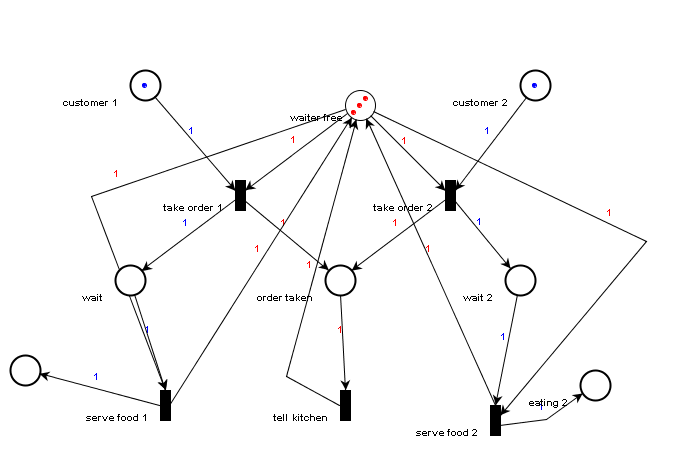
\includegraphics[width=450pt]{restaurant.png}
\label{restaurantnet}
\end{center}
\caption{An example of a behavioral model of a restaurant expressed in a Petri net}

\end{figure}

\section{Time Planning}
The essential extension to the situations framework that is proposed in this thesis adds an element of time to the system. This is needed to enable the system to deal with daily motion patterns. An important element without which the system cannot succeed is knowledge about how long actions are going to take. Only when this information is known to the agent (or system) it can be decided whether taking a certain action will result exceeding the deadline for the goal.


\section{Which Techniques Can We Use?}
We have seen many different techniques for many different purposes. We can immediately eliminate most global approaches to  crowds, since for most environments, we do not want the pedestrians to move as one big mass, all pedestrians heading into the same direction. Using purely attracting and repulsive forces will also generally not work when the pedestrians are too far apart, so we have another reason to rule out most global techniques. Of course, the global roadmaps approach does enable the pedestrians to split up and walk in different directions, but using this system on its own will not create very realistic behavior, since it does not have the capability to deal with interpersonal relations, and interaction with objects.
The techniques focusing on smaller groups do show some potential. Since most people move in smaller groups, this can lead to realistic effects. Ideally, people should interact with each other based on a variety of social relationships such as "parent" and "friend". However, this will require much configuration beforehand, and may increase processing time for each decision the pedestrians have to make. In this case, configuration may not be the issue, since these relationships can be defined and then used for many different simulations, but processing time is a larger problem, increasing with the number of pedestrians present in the simulation.
Of all the possible existing techniques, the "situations" approach of Sung et al. seems the most appealing. However, it is not directly usable for our purposes. One downside to the situations approach (at least how it is described in the paper) is that state transitions are mainly low-level animations. However, it should be possible to adapt the state transitions to correspond to higher-level actions, such as change of goal. Path planning should then be delegated to another module. In this way, it is very likely that the state representation can be reduced from $s = \{t, \bf{p}, \theta, s^- \}$ to $s = \{t, \bf{p}, \theta\}$. The $s^-$ was used to remember which actions were taken previously, so that the pedestrian remembers which way it was walking. When the actual walking is delegated to another module, it seems unnecessary to keep $s^-$.

\chapter{Method}
\todo[inline]{Check whole thesis on occurrence of "probability" function and replace it with "utility function" where necessary}
In the upcoming sections will be described how we decided to implement our system. We decided to base our model around the situations framework. We chose this framework because it allows for probabilistic behavior, and puts emphasis on defining behavior through the environment. This framework will have to be extended to deal with time restrictions. However, we won't work with finite state machines, as Sung et al. do, since these offer too little functionality to enable us to work with time restrictions. Furthermore, FSMs are not suitable for describing interactions between multiple agents. That is why we do the behavior modeling a little bit differently in our system. Instead of modeling the system with finite state machines, we describe the behavior of the pedestrians with Petri nets.  The toolkit we will use for this is \emph{Platform Independent Petri net Editor 2} (PIPE2). \url{http://pipe2.sourceforge.net/} Further down below we describe how we decided to use this toolkit.

In short, this chapter will describe how we combined the situations framework with Petri nets instead of finite state machines, and added a mechanism with which we compute a "utility" measure for behavior.

In our method, a number of concepts will be mentioned that have a vary specific meaning within our research. These concepts might sometimes be easily confused with each other.
\todo[inline]{Decide if this is the appropriate place to introduce these concepts}
\begin{itemize}
\item \emph{Scene}\\
A scene or scenario is the area where the simulation takes place. For example, in our experiments the scene is Rotterdam airport.
\item \emph{Situation}\\
In our research, the term situation is used to indicate an area in a scene where a specific behavior is appliccable. For example, a situation could be the area around a drinks machine.
\item \emph{Situation area}\\
The situation area is a part of the area of the scene where a certain situation is placed. Within this area the pedestrians will act out the behavior that belongs to this situation.
\item \emph{Behavior}\\
A behavior is a group of consecutive actions. In our framework a situation (as previously described) always has a accompanying behavior. The behavior for the drinks machine situation would be going up to the machine and buying a drink.
\item \emph{Action}\\
Actions are the building blocks in which a behavior is described.
\item \emph{Petri-net}\\
Petri-nets are the modelling language in which we describe our behaviors.

\end{itemize}

It is important to keep in mind the difference between behaviors and actions when covered in my theses. These two terms are not interchangable. With \emph{actions} we indicate movement of a pedestrian that is described in a single transition in a Petri-net. \emph{Behaviors} on the other hand, indicate the whole set of actions that are encompassed within a whole situation. Another way a behavior can be viewed is the whole sequence of actions that take place when a token of a pedestrians Petri net leaves the base place until it comes back again. \\
For example, a pedestrian might have entered the region of the toilet situation. A new \emph{behavior}, namely the Petri net corresponding to the toilet situation, is then attached to the pedestrian. A pedestrian might then decide to fire the transition that produces a token in this newly attached Petri net, thus making the pedestrian execute the behavior corresponding to the toilet situation. This Petri net consists of several transitions, corresponding to various \emph{actions}, such as walking to the toilet.


\todo[inline]{Extend introduction.}
\section{Petri-nets}
\todo[inline]{Make subsections}
Our method of designing behavior for large groups of pedestrians is largely based on the situation framework by Sung et al., but the finite state machines are replaced by Petri nets.

Stuff I should mention here:
\todo[inline]{Write this out but check if this is already mentioned in other parts of the method}
Our Petri-nets are based on place/transition Petri nets (p/t-nets). However, we did make some changes to the way one transition is selected from a set of enabled transitions. These changes were necessary to be able to incorporate a way of dealing with time pressure. In order to have the selection between enabled transitions change over time we compute a new set of probabilities at every timestep based on the rate (a standard property of transitions), the current time and our utility function. The details of how we decided to do this can be found in section \ref{timeplanning}.


Because a pedestrian should only be able to do behavior when he is in the associated situation, we should keep the Petri nets belonging to the pedestrian and the nets that describe the behavior for a situation separate. For a better idea about how we want to do this, see figure \ref{petrinetexample}. In the middle of this figure we can see the base place, to which all Petri nets eventually loop back, except for the gotogoal behavior. More about why we have restricted the Petri nets in this way can be found in section \ref{sec:restrictions}. The large circles in this example actually indicate the situation Petri nets. These have to attach to and detach from the pedestrian Petri net as he walks in and out of the associated situation. We do this through \emph{source} and \emph{sink} transitions. When a pedestrian walks into a certain situation, two new transitions of are attached to the base place. One of these transitions has an arrow pointed from itself to the base place, this is a source transition. The other transition, which as an arrow pointed the other way around is a sink transition. Because a source transition does not consume any tokens, but only produces one, it is always enabled so can fire at any time. Sink transitions only consume tokens. In our system, we treat these special source and sink tokens differently from other transitions. These newly generated transitions will be associated to sink and source transitions of the situation Petri net. This way, when a newly attached sink transition is fired in a pedestrian Petri net, the associated source transition of the situation Petri net will be found and fired as well. This way tokens can be "transported" from pedestrian Petri nets to situation Petri nets. Situation Petri nets have a fixed amount of special source and sink transitions, so no new ones are generated through the simulation. These sources and sinks indicate where a pedestrian Petri net should "attach" its sink and source transition when the pedestrian enters the associated situation. Whether a source or sink transition in a situation Petri net is meant to be attached to a pedestrian Petri net can be seen in the name of these transitions. These sources and sinks always come in pairs with the names $source:n$ and $sink:n$.
There is another way in which these source and sink transitions are treated differently. Regular source transitions are always enabled. Therefore, if these transitions would be treated as other transitions, attaching a situation to a pedestrian would create a transition that releases an endless amount of tokens into the Petri nets, which would upset our system. It is possible implement for example a situation in which a regular source transition is incorporated. Whether the system will work correctly is left to the judgement of the designer of the Petri net. An important rule is that a pedestrian net should always be able to transport only one token to a situation Petri net, and only one should be transported back.

\todo[inline]{Modify image \ref{petrinetexample}}
\begin{figure}
\centering
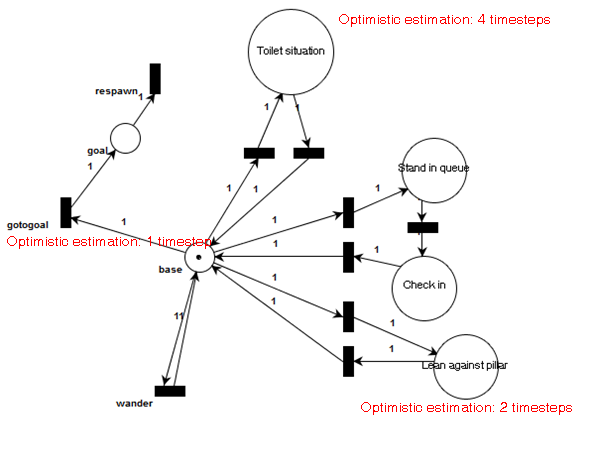
\includegraphics[width=350pt]{example}
\caption{Example structure}
\label{petrinetexample}
\end{figure}

%\todo[inline]{Is this the place to discuss PIPE2 or should it be placed in the appendix?} Here because having a toolkit to easily create those petri nets is pretty relevant.
PIPE2 is a tool written in Java to create and analyse petri nets. We chose this toolkit for a number of reasons. First of all, PIPE2 is written in Java, which makes it easier to integrate with our system. Secondly, this toolkit promised a number of Petri net extensions, the most important of which is the capability to create \emph{Generalized Stochastic Petri nets}. Generalized stochastic Petri nets is an extension that adds timed transitions to the modeling language. Most importantly, PIPE2 provides a clear and simple GUI with which Petri-nets can be designed. This is very important because the design of the behavior in our method should be fast and easy. It should require minimal effort to place large amounts of agents in a environment.
%\todo{Name other reasons, since we don't use generalized stochastic petri nets any more}
Unfortunately, at a later time it seemed that the generalized stochastic petrinets that we planned to use did not behave as described in the specifications, so that is one of the reasons we stick to use modified, basic, place/transition Petri nets.  
%\todo[inline]{Name disadvantages? Most disadvantages only become clear after PIPE2 has been used for a while so choosing PIPE was mostly because there was not enough time to extensively study alternatives, but it shouldn't be put like that.}



%This can be done by replacing the regular probabilistic finite state automata with probabilistic \emph{timed} state automata. Furthermore, we will be building an additional layer on the situations framework which will deal with with the \emph{needs} of the pedestrians. The list of needs a pedestrian will have will be dependent on which needs are defined in the situations in the environment. If, for instance, the environment contains a "food stand" situation, in which is specified that it defines the "hunger" need, pedestrians will act on this need. Whereas when the pedestrians are placed in an environment where for instance no food stands exist, and the "hunger" need cannot be fulfilled, pedestrians will not have this need at all.


%\section{Pedestrian Layer}
%Some drastic changes will be made in order to adapt the situations framework to our needs. Instead of using regular finite state automata, we use Petri nets so that environments in which time constraints are important (e.g. train stations, airports, etc. ) can be properly dealt with.

\todo[inline]{Commented out quite some text because PIPE2 did not work as promised. Replace this text by text that does describe how we actually used the Petri nets. Maybe some of the text is still usable? Also, check if this text shouldn't be further down below, or maybe it is already there.}

%\subsubsection{Probabilistic Timed State Automata}
%In the approach of Sung et al., regular probabilistic finite state automata are used. However, this is not sufficient when dealing with time-constrained goals. This is why we use a system called probabilistic timed automata. Probabilistic timed automata are an extension to B\"{u}chi automata which in turn are an extension to finite state automata. B\"{u}chi automata extend finite state automata to infinite inputs. Probabilistic timed automata use the acceptance conditions used in B\"{u}chi automata and extend these by using clocks, which can be incremented or reset. These clocks can be incorporated in the acceptance conditions, so that %transitions can be restricted based on time.

%\subsubsection{Time Planning}
%Our most important addition to the situations framework will be the aspect of time planning. This is going to be realised by %restricting the petrinets to follow a certain structure, so the time to the goal can be computed with the guarantee that a %path to the goal can be found relatively fast
%\todo[inline]{Elaborate on "fast"}
%Our approach is centered around the idea that the Petri nets designed for the standard pedestrian behavior all include a %"base" place. All regular tokens have to eventually return to this base place. Another important aspect of this place is that it %is directly connected to the transition that leads to the goal place. This way, searching for sequences of behaviors leading %to the goal place in time is greatly simplified.

%\todo[inline]{Refine following text}
%The general gist is that we use the idea of Beauquiers probabilistic timed automata \cite{Beauquier03}. Which means we %assign clocks to transitions and a transition is only accepted when the clock condition holds, and we use probabilistic %transitions, but we wont use the whole MDP problem solving part.

\section{Restrictions and Assumptions}
\label{sec:restrictions}
\todo[inline]{Maybe put more at beginning?( Or at end of method)}
The method we propose is based on various restrictions which have to be clarified. An important restriction is that the environment the pedestrians have to walk in are designed in such a way that it helps creating realistic behavior. This means that situations have to be defined in such a way that pedestrians will walk into them and act in the appropriate way. This makes our framework probably limited to certain kinds of environments. If a situation is appropriate in the entirety of the scene though, a situation can be designed with an area that encompasses the whole area of the scene. When an environment does not contain many situation areas or if they are too far apart, it is very likely that the framework does not give a satisfactory result.
An important assumption that we make about the scenes that our system has to model is that the pedestrians have to be at a certain place at a certain time. This makes the system more suitable for daily routine type situations rather than cases in which pedestrians are walking around without a proper goal. However, most situations can be described as having a deadline (e.g. eventually, most people have to go to bed), so this assumption is not necessarily very restrictive.\\
Furthermore, we assume that it is possible to describe the behavior of the pedestrians in Petri nets, and that these models incorporate \emph{base places} to which all ¨paths" eventually loop back, and from which it is always possible to reach the "goal place" (given enough time is left) We need this assumption in order to create an efficient way of determining which actions can be done before the deadline. \\
\todo[inline]{Add restriction that one token should go to situation and back}

\section{Preparations}
In order to save computing time during a simulation, we make a few computations before the simulation has started, to use during the simulation. An important step is the calculation of the distance in time between all the places in a Petri net and a destination place (such as the goal place). This distance can easily be computed using the \emph{Dijkstra shortest path algorithm} \cite{dijkstra}. Dijkstra's algorithm is a graph search algorithm that can produce a shortest path tree for a single source, for a graph with nonnegative edges. In our system we can use this to compute the time from any place to the destination place (the source). This can be very useful when we would like to compute an estimate of how long a pedestrian will be stuck to the behavior of a certain situation. However, it will never be more than an estimate, since it is possible to design Petri nets with (possibly) infinite loops. But since the Petri nets are probabilistic, it will never be possible to give an exact prediction of the time it takes to execute a certain behavior.

The use of Dijkstra's algorithm does limit the use of our Petri nets though. For our simple implementation of Dijkstra's algorithm to be effective, we cannot use the Petri nets' more advanced features such as colored tokens. When a Petri-net has colored tokens, a different treatment can be defined for these different tokens. They are able to reach the same places, but 

\todo[inline]{Write about problems with dijksta and petri nets, such as multiple tokens/slots, and colored tokens etc.}

\section{Time Planning \& Decision Mechanism}
\label{timeplanning}
The fact that we use Petri nets with timed transitions instead of finite state automata does not necessarily mean our pedestrians are able to deal with time constraints. However, these Petri nets have helped making our problem representable. In order to use these stochastic Petri nets efficiently for making decisions based on time constraints, we have made a number of assumptions.\\
First of all, we assume there are certain \emph{base places} from which it is always possible to reach the (time constrained) goal. Then, we will compute for every transition that will not take the pedestrian to its goal, how much time it takes to get back to the base state. Then we can check whether the goal place is still accessible from the base state when a certain transition has been taken. We use this information to modify the timed transition rate, so pedestrians are more likely to choose the actions that leave them more time to reach their goal.
As one may have noticed, this approach does not give a completely watertight solution to the planning problem. However, since we have to be able to model large crowds, we cannot create an overly complex planning system, since we would not be able to run the simulation real-time. Furthermore, we do not aim at finding an optimal solution to the planning problem, but rather the most lifelike behavior. In real life, people make errors in judgement, so creating pedestrians who can look ahead perfectly would not be realistic. It is impossible to make an exact definition of realism for our purposes, but what we try to do, is to copy certain specific behavior found in real-life footage. In our experiments we will try different functions for computing the probability of going to the goal, and attempt to assess which function will be most suitable.
\todo[inline]{About the most important part of the thesis, so has to be extended}
\todo[inline]{Include Pictures}



\subsection{The Basic Algorithm}
Though the probabilities of the various behaviours a pedestrian can have is dependent on what kind of distribution we are going to use, the underlying mechanism will always be as described in algorithm \ref{decisionmechanism}. This algorithm is used to choose one of the various behaviors that are currently available to a pedestrian at a certain timestep. Once it is chosen, this behavior will be executed be executed in the following timesteps. This algorithm is only run for the pedestrians whose token is currently in the base place. When the token is in another place, the decision about which transition to choose follows the basic Petri net rules.\\
First of all, we subtract the current time from the deadline time of the pedestrian.  Before we go any further, it is important to understand how we keep track of the time. \todo[inline]{Achterhaal of iedere pedestrian een persoonlijke time heeft of dat er een algemene timer is. Ik ga voorlopig uit van een persoonlijke timer ook beslissen of het volgende detail misschien meer een implementatiedingetje is.} Every pedestrian has its own timer which in our system is implemented to increment by one at every timestep of our simulation engine. When we have computed $t_d$, we know how much time the pedestrian has left to reach its goal.\\
Next, the algorithm computes for every situation how much time is left would the pedestrian choose and execute this behavior. This remaining time is then used to compute the probability rate of the pedestrian deciding to choose this behavior. The probability rate is computed with the function $\phi$, and can have various distributions. In chapter \ref{chap:experiments} (\emph{Experiments}) we will try out various options for $\phi$ to see which will give the most realistic behavior. When the probability rates for all the behaviors have been computed, they are normalized, and based on the resulting probabilities, one of the behaviors is randomly chosen.

\todo[inline]{Check if it's the right way around (afteller of opteller)} 
\todo[inline]{Improve structure}
\begin{figure}
\begin{algorithm}
\caption{The behavior decision mechanism}
\label{decisionmechanism}
\begin{algorithmic}
\State $t_d \gets $ deadline time - current time 
\For{Every connected situation}
\State $t_e \gets $ estimated time for situation
\State $\tau \gets t_d - t_e$
\State Probability rate $\gets \phi(\tau))$
\EndFor
\State normalize(probability rates)
\State select one transition according to the computed probabilities
\end{algorithmic}
\end{algorithm}
\end{figure}

\section{Rotterdam Airport}
In our research, we focus on behavior found at Rotterdam airport. In order to know what the behavior at this location looks like, we have observed footage from the security cameras at Rotterdam airport. From these observations we have established a couple of specific behaviors that are recurrent in Rotterdam airport.
\todo[inline]{How often do these behaviors occur?}

\begin{itemize}
\item \emph{Going to the toilet.}
\\In the videos, we observed that a typical behavior that manifests itself multiple times in the video material is that one person goes to the toilet, and another one waits until this person has come back. After that, they move on to do something else. The Petri-net can be found in figure
\todo[inline]{If I have time I could modify the implementation of this behavior so that the pedestrian actually goes back to his friend after going to the toilet, or at least to the place where he came from}
\todo[inline]{I removed the "checking in" behavior because it was difficult to implement. Maybe if I have some time left I will give it another try because it is quite important behavior for an airport}

\item \emph{Leaning against a pillar.}
\\Another recurring behavior we saw is that people lean against the pillars in the hall. 

\item \emph{Wandering}\\
People also wandered around randomly.
\end{itemize}
\todo[inline]{If I introduce the behavior here I can't talk about them yet in the method. Check if I do this}

We managed to recreate the behavior in the Petri nets in figure \ref{fig:pillarpetrinet}, \ref{fig:standstillpetrinet}, \ref{fig:gototoiletpetrinet} and \ref{fig:wanderpetrinet}. As can be seen, the ¨standing still¨ behavior in figure \ref{fig:standstillpetrinet} was easiest to recreate, closely followed by the "wandering" behavior in figure \ref{fig:wanderpetrinet} and "leaning against a pillar" behavior. The exact appearance in the simulation mostly depends on the implementation of the actions indicated in the places of the Petri nets. Whether there will be e.g. collision detection or other lower-level functionality depends on which kind of multiagent simulation is used. The "go-to-toilet" behavior in figure \ref{fig:gototoiletpetrinet} is the most interesting, because this Petri net can actually be shared between two pedestrians. We see that this fairly complicates the structure of the Petri net. In comparison to the other Petri nets, there are relatively more places here that do not map to an actual action. These places are necessary to make sure that one pedestrian does not move forward to its next action too soon. This will cause the pedestrians to have more "idle" actions between their other actions than there would be with the simpler behavior. This is not a problem though, because the pedestrians will not remain idle longer than one or two timesteps.

\todo[inline]{Check gototoilet Petri one last time to see if there aren't any redundant places/transitions}

\begin{figure}
\centering            
\includegraphics[width=0.7\textwidth]{/home/djura/vakken/svn_afstudeerstage/deadline-driven-behavior/report/petrinet_pictures/pillarSituation.png}
\caption{Going to the nearest pillar and leaning against it.}
\label{fig:pillarpetrinet}
\end{figure}

\begin{figure}
\centering            
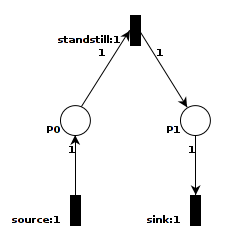
\includegraphics[width=0.4\textwidth]{/home/djura/vakken/svn_afstudeerstage/deadline-driven-behavior/report/petrinet_pictures/standStillSituation.png}
\caption{Pedestrian standing still.}
\label{fig:standstillpetrinet}
\end{figure}

\begin{figure}
\centering            
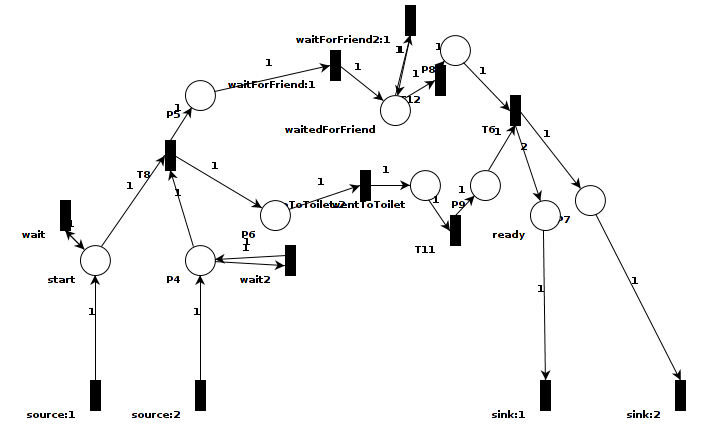
\includegraphics[width=\textwidth]{/home/djura/vakken/svn_afstudeerstage/deadline-driven-behavior/report/petrinet_pictures/twoPeopleToiletSituation.png}
\caption{One person going to the toilet and one person waiting for the other.}
\label{fig:gototoiletpetrinet}
\end{figure}

\begin{figure}
\centering            
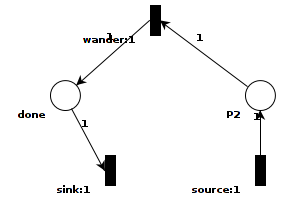
\includegraphics[width=0.5\textwidth]{/home/djura/vakken/svn_afstudeerstage/deadline-driven-behavior/report/petrinet_pictures/wanderSituation.png}
\caption{Random wandering around}
\label{fig:wanderpetrinet}
\end{figure}

\section{Example}
\todo[inline]{Check if the title of this subsection is ok}
Figure \ref{petrinetexample} gives an example of how the pedestrian petrinet is connected to the situations. It also shows the estimation created by the Dijkstra preprocessing algorithm that makes a guess at how much time it takes to complete the situation behavior. This is the value that will be used when computing the time at which the token of a pedestrian will move back to its base place.

In order to give a clear insight into how our method is used in practice we will give a small example. Let us say that we need to simulate only one person, who has to wait in a room. At a certain point in time (let us say 100 steps), he has to advance through a door. There are a few objects in this room with which he can interact. \ref{fig:roomwithagent} and \ref{fig:roomwithagentsituations}

\begin{figure}
\centering
\begin{subfigure}[b]{0.5\textwidth}
\centering
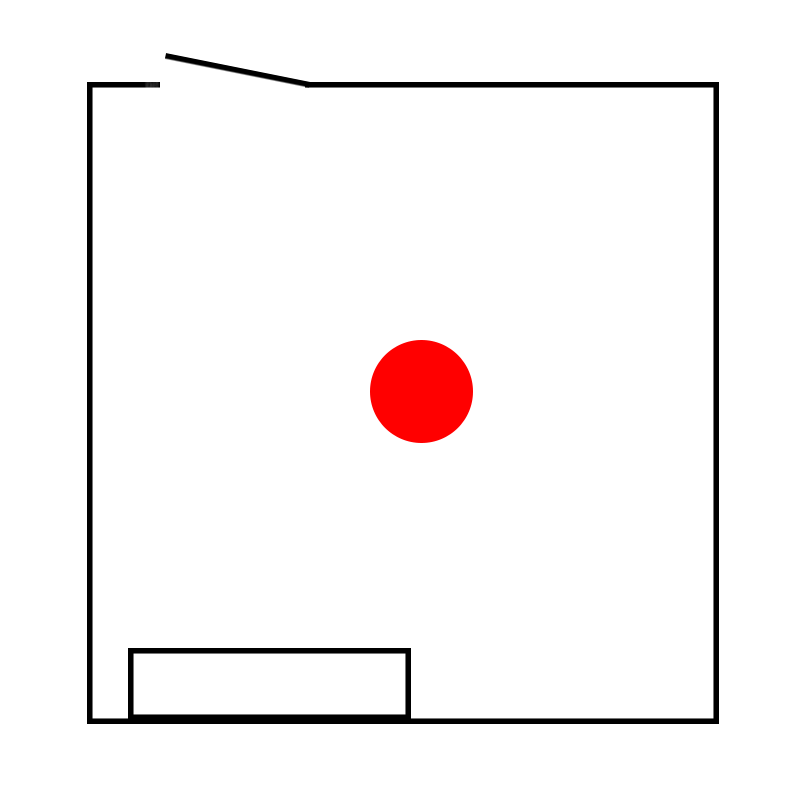
\includegraphics[width=.4\textwidth]{/home/djura/vakken/svn_afstudeerstage/deadline-driven-behavior/report/room_with_agent.png}
\caption{Room with agent}
\label{fig:roomwithagent}
\end{subfigure}%
\begin{subfigure}[b]{0.5\textwidth}
\centering            
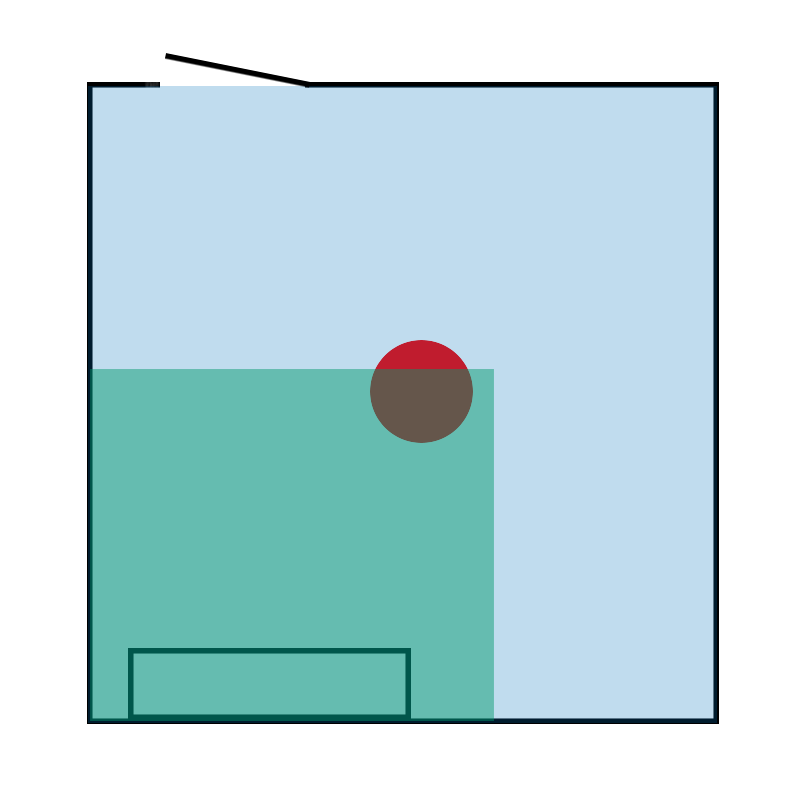
\includegraphics[width=.4\textwidth]{/home/djura/vakken/svn_afstudeerstage/deadline-driven-behavior/report/room_with_agent_and_situations.png}
\caption{Room with agent and situation areas.}
\label{fig:roomwithagentsituations}
\end{subfigure}
\caption{A hypothetical room that could be simulated.}
\end{figure}

\chapter{Experiments}
\label{chap:experiments}
\todo[inline]{Add pictures of the Petri nets}
\todo[inline]{Make sure introduction lines up with research questions}
Although it can be difficult to decide whether a group of people walks around "realistically", we will certainly give it a try. We will attempt to test our framework in two different ways; first of all, we will assess our framework by doing a qualitative comparison with real-life footage of Rotterdam Airport. We have access to both camera footage and manually tracked locations of the visitors.
\todo[inline]{Check whether I still use the manually tracked locations, otherwise I shouldn't mention it.}
Secondly, we will assess how the the different utility functions we choose for the go-to-goal action will affect the frequency of other actions. In other words, we will attempt to investigate whether our method leads to \emph{emergent} behavior.

\todo[inline]{Specify missing parameters}

\section{Qualitative Experiment}
First of all, we will see if it is possible to recreate real-life behavior in Rotterdam airport with our framework. In order to do this, we have observed footage from the security cameras at Rotterdam airport. From these observations we have established a couple of specific behaviors that are recurrent in Rotterdam airport:

\begin{itemize}
\item \emph{Going to the toilet.}
\\In the videos, we observed that a typical behavior that manifests itself multiple times in the video material is that one person goes to the toilet, and another one waits until this person has come back. After that, they move on to do something else. This will probably be the behavior in our simulation that will take the largest amount of time.
\todo[inline]{If I have time I could modify the implementation of this behavior so that the pedestrian actually goes back to his friend after going to the toilet, or at least to the place where he came from}
\todo[inline]{I removed the "checking in" behavior because it was difficult to implement. Maybe if I have some time left I will give it another try because it is quite important behavior for an airport}

\item \emph{Leaning against a pillar.}
\\Another recurring behavior we saw is that people lean against the pillars in the hall. 

\item \emph{Wandering}\\
People also wandered around randomly.
\end{itemize}
\todo[inline]{If I introduce the behavior here I can't talk about them yet in the method. Check if I do this}

It will be difficult to assess whether our framework simulates ¨real-life¨ in some way or another, but we can find out whether it is possible to describe the behaviors we found in real life in Petri-nets. We will show if our framework can do this.
\todo[inline]{Experiment has to be changed. In experiments, give indication of how often the behaviors take place, how often do they take place in simulation? Also look at trajectories of these behaviors and compare with trajectories of simulation.}

%One crucial behavior is missing. How are the pedestrians going to reach the different situation areas? This is only possible if they already have a move to begin with, otherwise they are only going to stay in place. That is why we added the \emph{fastWander} and \emph{slowWander} behavior. This behavior lets the pedestrian turn a random amount of degrees between $-\frac{1}{4}\pi$ and $\frac{1}{4}\pi$ and walk a few steps in that direction. Of course, fastWander makes the pedestrian move faster than slowWander, and takes less time. Another important reason we have added these two behaviors is that we can use them to see more clearly if relaxed or hurried behavior is favored differently over time.


%\paragraph{Standing in the queue for the check-in desk}
%\todo[inline]{This paragraph should probably be removed since we dont use it any more}
%One constant factor in the video material seemed to be the people lining up in front of the check-in desk. There are many ways to %model this behavior with our framework.
%\todo{Mention other ways to model this}
%We decided to split this behavior in two situations. First of all, we have the check-in situation, which in our simulation comes down %to standing in front of the check-in desk for a short period of time. The other half of this behavior is the queue situation. This is an %area in the hall where people line up with the people in front of them. The situation area is chosen such that the pedestrians in it %will together form an orderly line. This means that the situation should not be too broad.


%\subsubsection{Checking in}
%When the pedestrians reach the end of the queue situation, they will enter the check-in situation, in which they will stand in front of the check-in desk for a little while, after which they are free to go again.


\section{Quantitative Experiment}
\todo[inline]{Check which parts of the first quantitative experiment are still relevant now the experiments have changed.}
It is very difficult to quantitatively establish whether lifelike behavior has been modeled. However, it is possible to check whether the mechanics of time planning work as predicted. In order to do this, we log for every step in time, for every pedestrian, which action he is doing at the moment. This information will be plotted in a graph that shows the frequency of every action at every step in time. The deadline of going to the goal will be 200 steps in our simulation. We chose this value because our behavior takes up to roughly 40 steps (but most behavior takes 20 steps or less) and this leaves enough room for the pedestrians to decide on multiple behaviors while "relaxed" before time starts running out and they have to start hurrying.
We will try different utility functions for the go-to-goal and non-goal behavior to see how this influences the simulation. The parameters for these functions have been decided on beforehand. We based our decision on what parameters would give a significant but gradual increase in the course of this timeframe and give the maximum utility on either $t=0$ or $t=200$, the first when the function is used as utility measure for go-to-goal behavior, the latter when applied to non-goal behavior. The utility functions will be judged on whether they result in behavior that transitions from relaxd to hurried, and whether they help the pedestrians reach their goal in time.

\subsection{Sigmoid Function}
A sigmoid function is an S-shaped curve that has a progression that accellerates and approaches a climax over time. This function can be found in many natural processes, such as learning curves. This function closely resembles how we reason that the behavior will shift when a pedestrian approaches a deadline.
Our sigmoid function is defined as follows:
\begin{equation}
U(\tau) = \eta \frac{1}{1+e^{-\omega(\tau-\tau_0)}} + \beta
\end{equation}
\todo[inline]{Check if the following parameters are still true}
In our experiments, we chose $\tau_0=100$ and $\omega=100$, so that the middle of the curve lies in the middle of the 200-timestep period which the pedestrians have to reach their deadline. We chose $\omega$ to be 100 as well to scale the function to fit in the 200 timestep interval. For $\eta$, we varied this between 0 and 1.
% When the deadline is far away, it does not matter much whether the pedestrian goes straight to its goal or does something else. Even if time shifts a little, it still does not matter much. However, when the pedestrian moves on

%\begin{figure}
%\centering
%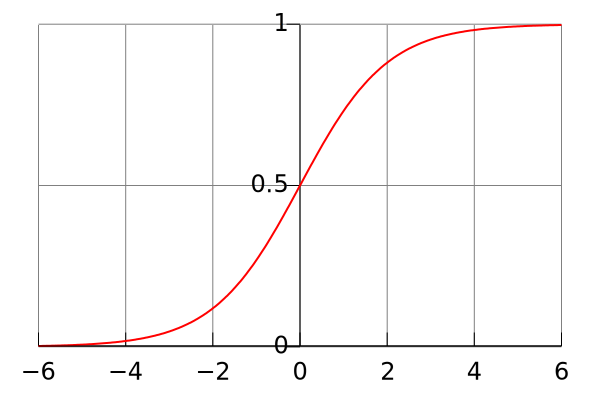
\includegraphics[width=200pt]{Logistic-curve}
%\caption{A typical sigmoid function}
%\label{sigmoid-example}
%\end{figure}

\subsection{Linear Function}
We first chose to use a sigmoid function, because intuitively it felt like it would reflect real-life behavior best. However, it could be the case that the sophistication of this function is lost in practice. If this is the case, we might as well use the simpler linear function. We will use this function to check the necessity of the sigmoid function. Our linear function was of the following form:
\begin{center}
If $0 \leq \tau \leq n$: $P(\tau) = a\tau + b$\\
If $\tau<0$: $P(\tau) = P(0)$\\
If $\tau<n$: $P(\tau) = P(n)$
\end{center}
However, we do not specify these parameters directly. What matters the most to us, is the value at the start of the linear utility function, $U$ at $\tau=0$, which we call $U_0$ and the value of $U$ at the end where $\tau=n$, which we call $U_n$. Consequently, we compute $a$ and $b$ as follows:
\todo[inline]{Check whether I'm consequent in the indication of the parameters and if it is correct to call the x axis $n$}
\begin{center}
$a = \frac{U_n - U_0}{n}$\\
$b = U_0$
\end{center}



\subsection{Gaussian Function}
We also used a Gaussian function to model the behavior, defined as follows:
%\begin{equation}f(x) = ae^{- \frac{(x-b)^2}{2c^2}}\end{equation}
\begin{equation}f(\tau)\frac{1}{\sigma \sqrt{2 \pi}} e^{- \frac{(\tau - \mu)^2}{2\sigma^2}}
\end{equation}
%Where real constants $a, b, c > 0 $. 
A Gaussian distribution (or normal distribution) is a continuous probability distribution with a bell-shaped probability density function which have a mean ($\mu$ and variance ($\sigma^2$) as parameters.
We chose to try a Gaussian function as well because of the following reasoning: A pedestrian might not care about going to it's goal until it is approximately the time of the deadline. With this we mean that going to the goal is a priority \emph{around} the time of the deadline, and will also decline when the deadline has passed for a while, and the pedestrian hasn't reached its goal yet. With this reasoning, the "go-to-goal" behavior frequency should increase when approaching the deadline, and should peak \emph{just} before the deadline, and declines thereafter.



\section{New Quantitative Experiment}
\label{sec:quantitativeexp2}
\todo[inline]{Part of this text can be moved to the first quantitative experiment, because that experiment now also includes slow and fast wander}
Because of newly discovered limits to our system that become clear in our results \ref{chap:results}, we decided to add new quantitative experiments. It turn out that with our previous quantitative experiments, the cumulative probability for going to the goal becomes so high in quite a few steps, that it is difficult to see any effect of our system on hurried and relaxed behavior. Very soon in most of our simulations, the number of pedestrians that have already reached to goal becomes so high that nothing valuable can be said of the other behaviors. That is why we have decided to run experiments where we have removed the behavior of going to the goal. We did this by simply removing the connection from the base place of the pedestrian to the gotogoal transition.
We also replaced the "wander" behavior by two other behaviors signifying hurried and relaxed behavior, called \emph{fastwander} and {slowwander}. We use these two behaviors to try to get a clear distinction between hurried and relaxed, and see how the number of pedestrians doing one or the other changes over time. The petri nets for these behaviors look exactly the same, as can be seen in figure \ref{fig:newSituations}. The difference between these Petri nets is in the weight of the slowwander:1 and fastwander:1 transitions. These are 20 versus 10 respectively. This weight is used in the system to compute the amount of time that a certain behavior will take. The reason that these are 20 and 10 is that we programmed the slowwander behavior in such a way that the pedestrian will walk roughly in one direction for 20 timesteps. Fastwander makes the pedestrian walk faster than slow wander, and for a shorter period of time, namely 10 timesteps. We added slowwander and fastwander situation areas, both encompassing the entire scene.

The experiment run as follows. At every timestep, every pedestrian logs what action it is currently doing. This log is then rearranged into a table where we have for every timestep, for every action the amount of pedestrians that are currently executing it. The results are then displayed in a graph. The results can be found in the next chapter in section \ref{sec:secondquantitativeexperimentresults}.

For this experiment, the following actions can be executed:
\begin{itemize}
\item \emph{fastwander}
\item \emph{slowwander}
\item \emph{gototoilet} and \emph{waitforfriend} (these both belong to the gototoilet situation)
\item \emph{gotonearestpillar} and \emph{leanagainstpillar} that are both part of the leanagainstpillar situation \todo[inline]{I just modified leanagainstpillar so it actually takes a few steps, otherwise it's hardly noticable. Should I rerun the experiments, or maybe just don't mention this behavior because it is not important?}|
\item \emph{standstill}
\item \emph{idle}
\end{itemize}
The last action is the default action when nothing else can be executed. It is executed when a fired transition does not have an associated action. Another situation in which this idle behavior can happen that will be important in these experiments, is when there are no transitions left anymore to fire. This can be for example when all transitions have gotten a probability of 0 for firing.

%\begin{figure}
%\centering
%\includegraphics[width=150pt]{"rotterdamPedestrianNet_secondexperiment"}
%\caption{The pedestrian Petri Net for the second quantitative experiment.}
%\label{fig:second_rotterdampedestriannet}
%\end{figure}

\begin{figure}
        \centering
        \begin{subfigure}[b]{0.5\textwidth}
                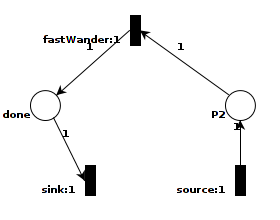
\includegraphics[width=\textwidth]{fastWanderSituation}
                \caption{"Fast wander" behavior.}
                \label{fig:fastWanderPetrinet}
        \end{subfigure}%
        ~ %add desired spacing between images, e. g. ~, \quad, \qquad, \hfill etc.
          %(or a blank line to force the subfigure onto a new line)
        \begin{subfigure}[b]{0.5\textwidth}
                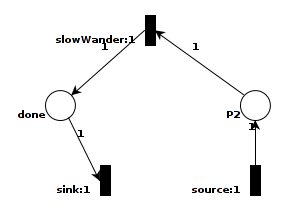
\includegraphics[width=\textwidth]{slowWanderSituation}
                \caption{"Slow wander" behavior.}
                \label{fig:slowWanderPetrinet}
        \end{subfigure}
        \caption{Petri nets of the new behaviors}\label{fig:newSituations}
\end{figure}

\todo[inline]{Show the difference between the pictures in \ref{fig:fastWanderPetrinet} and \ref{fig:slowWanderPetrinet}, color the upper transitions red and show they have a different rate.}

\chapter{Results}
\label{chap:results}

\section{Results of the Qualitative Experiment}
\label{sec:qualitativeresults}
\todo[inline]{Rewrite results of qualitative experiment}
\todo[inline]{Show GUI! how do the pedestrians walk?}

%\todo[inline]{The following is only a rough draft}
%It is very difficult to determine whether one has been successful at modeling lifelike behavior. What we are going to do is %study footage of real-life behavior at Rotterdam Airport, and pick out various behavioral patterns. Then, we are going to %model these patterns with our system.



\section{Results of the First Quantitative Experiment}
\label{sec:firstquantitative}
Firstly we are going to discuss the results of the first quantitative experiment. One thing that is noticable in all results is that there are periods in which the number of pedestrians, especially in slow and fast wander, is steady, after which the number drops drastically. After a few steps the number goes up again. In sync with this behavior the number of pedestrians remaining idle stays low, and increases when the other behaviors drop. This is easily explained. Slow and fast wander are behaviors that exist of a single action. When this action has been executed, which takes a few steps, the token of the pedestrian moves out of the attached Petri net into its base place. In order to move this token, a slot and sink transition have to be fired. These transitions do not have an associated action. When there is no action available for the pedestrian, it executes the idle behavior. Especially at the start, this effect is very prominent. This is because all pedestrians start the simulation at exactly the same moment. All pedestrians executing the same actions or actions that take the same amount of time stay synchronous. After a few dozens of steps, the behavior has varied more and the pedestrians are not as synchronous any more in going back to the idle "action".

Another thing that we can notice is that there are more or less four actions that dominate simulation, namely \emph{slow wander}, \emph{fast wander}, \emph{go to goal}, and \emph{idle action}.
\todo[inline]{What happened to lean against pillar?} Behavior like going to the toilet and waiting for their friend (which are both part of the same going to the toilet behavior and Petri-net) are only done by one or two pedestrians at a time. This is completely as expected. The go-to-toilet situation is shared, which means that one Petri-net is attached to multiple pedestrian Petri-nets. The more dominant actions belong to situations that are not shared and are instantiated for every pedestrian that enters it. That means that the shared Petri nets are only instantiated once for every situation, while the ones that aren't shared are instantiated many times.

In figure \ref{fig:linear0to1goal1to0}, \ref{fig:sigmoid100_0_10_1_goal1to0} and \ref{fig:Gaussian200_50_1_goal1to0} we see the results for having a linear goal utility function that decreases from 1 to 0 and the utility function for other behavior varying. Figure \ref{fig:linear0to1goal1to0} and \ref{fig:sigmoid100_0_10_1_goal1to0} look very similar. The simulation starts out with a large preference for slow wander behavior, which decreases while fast wander increases. After about 70 steps however, the gotogoal action starts to dominate the simulation, increasing at a fast pace. This makes the other actions decrease rapidly until pedestrians are either idle (because they have already reached their goal) or still going to their goal. When we look at figure \ref{fig:Gaussian200_50_1_goal1to0} we see that almost all pedestrians go to the goal in the first dozen of steps. Fast wander and slow wander become completely overshadowed.


\begin{figure}[h!]
\centering            
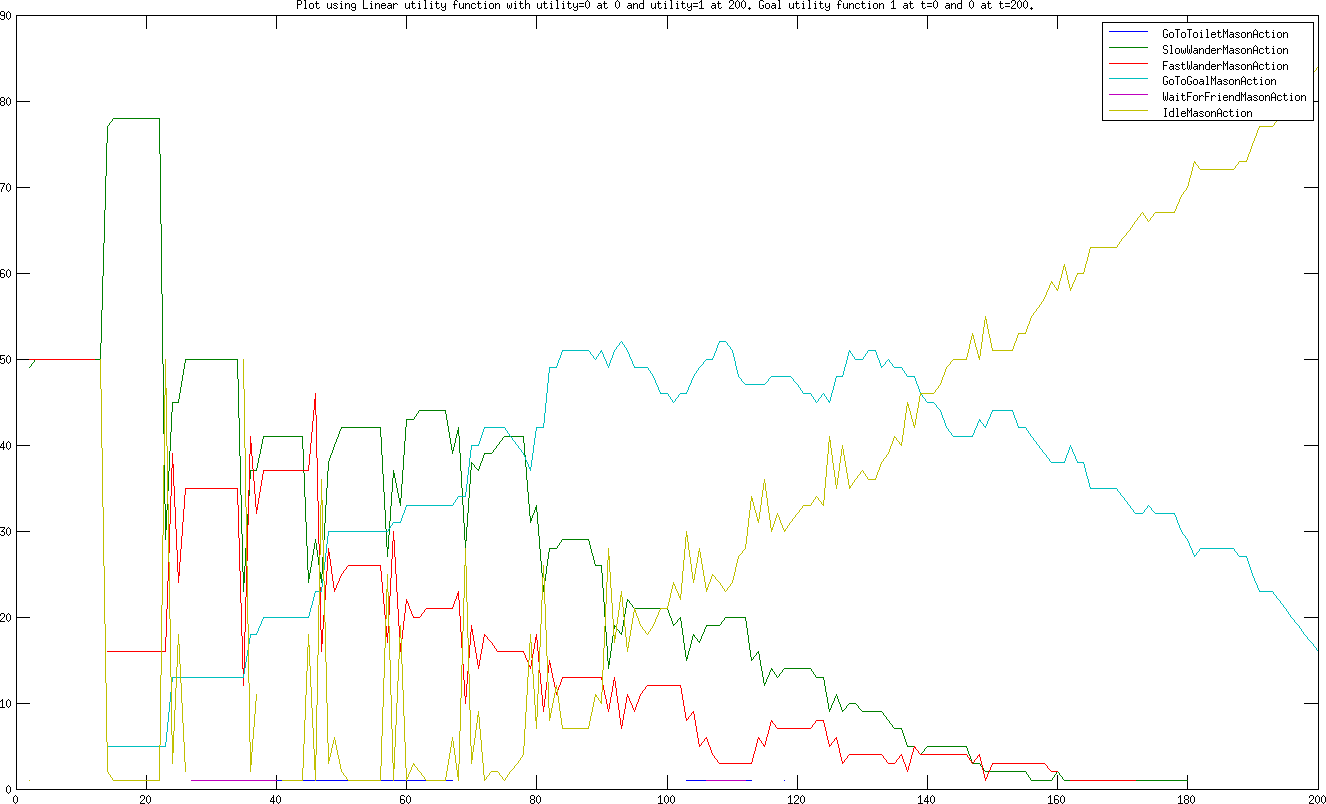
\includegraphics[width=\textwidth]{/home/djura/vakken/svn_afstudeerstage/deadline-driven-behavior/hulpscriptjes/goodresults/linear0to1goal1to0.png}
\caption{Goal utility linear with $U_0=1$ and $U_n = 0$. Other behavior utility linear with  $U_0=0$ and $U_n=1$.}
\label{fig:linear0to1goal1to0}
\end{figure} 

\begin{figure}[h!]
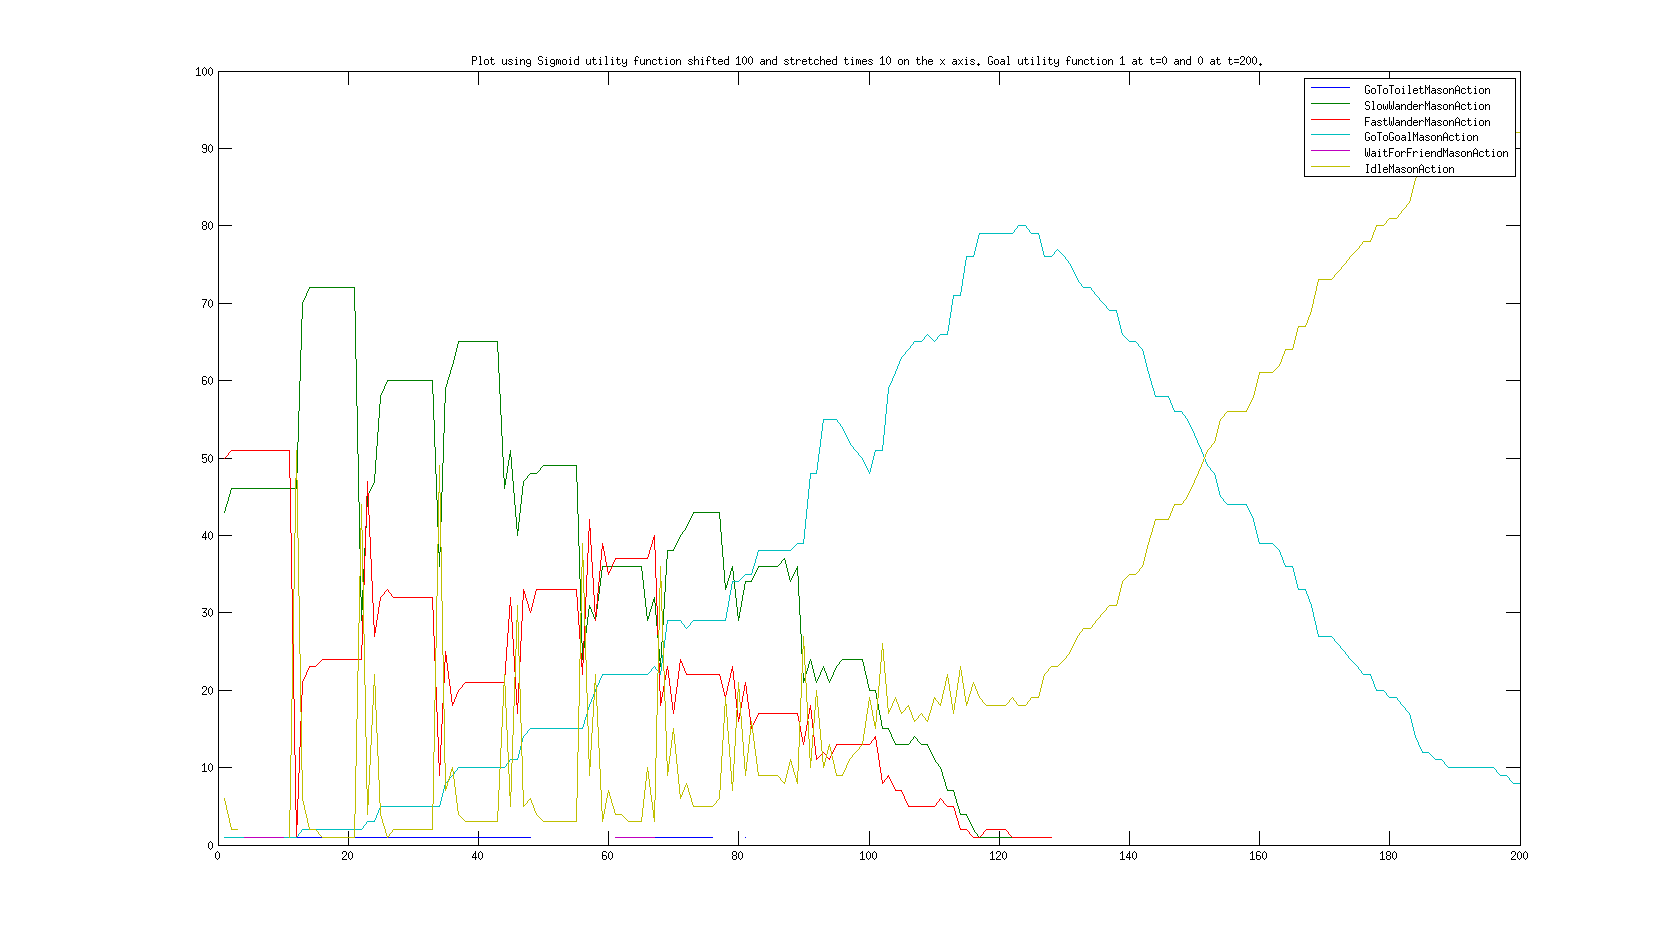
\includegraphics[width=\textwidth]{/home/djura/vakken/svn_afstudeerstage/deadline-driven-behavior/hulpscriptjes/goodresults/sigmoid100_0_10_1_goal1to0.png}
\caption{Goal utility linear with $U_0=1$ and $U_n = 0$. Other behavior utility sigmoid with $t_0=100$ $\beta=0$ $\omega=10$ $\eta=1$}
\label{fig:sigmoid100_0_10_1_goal1to0}
\end{figure}

\begin{figure}[h!]
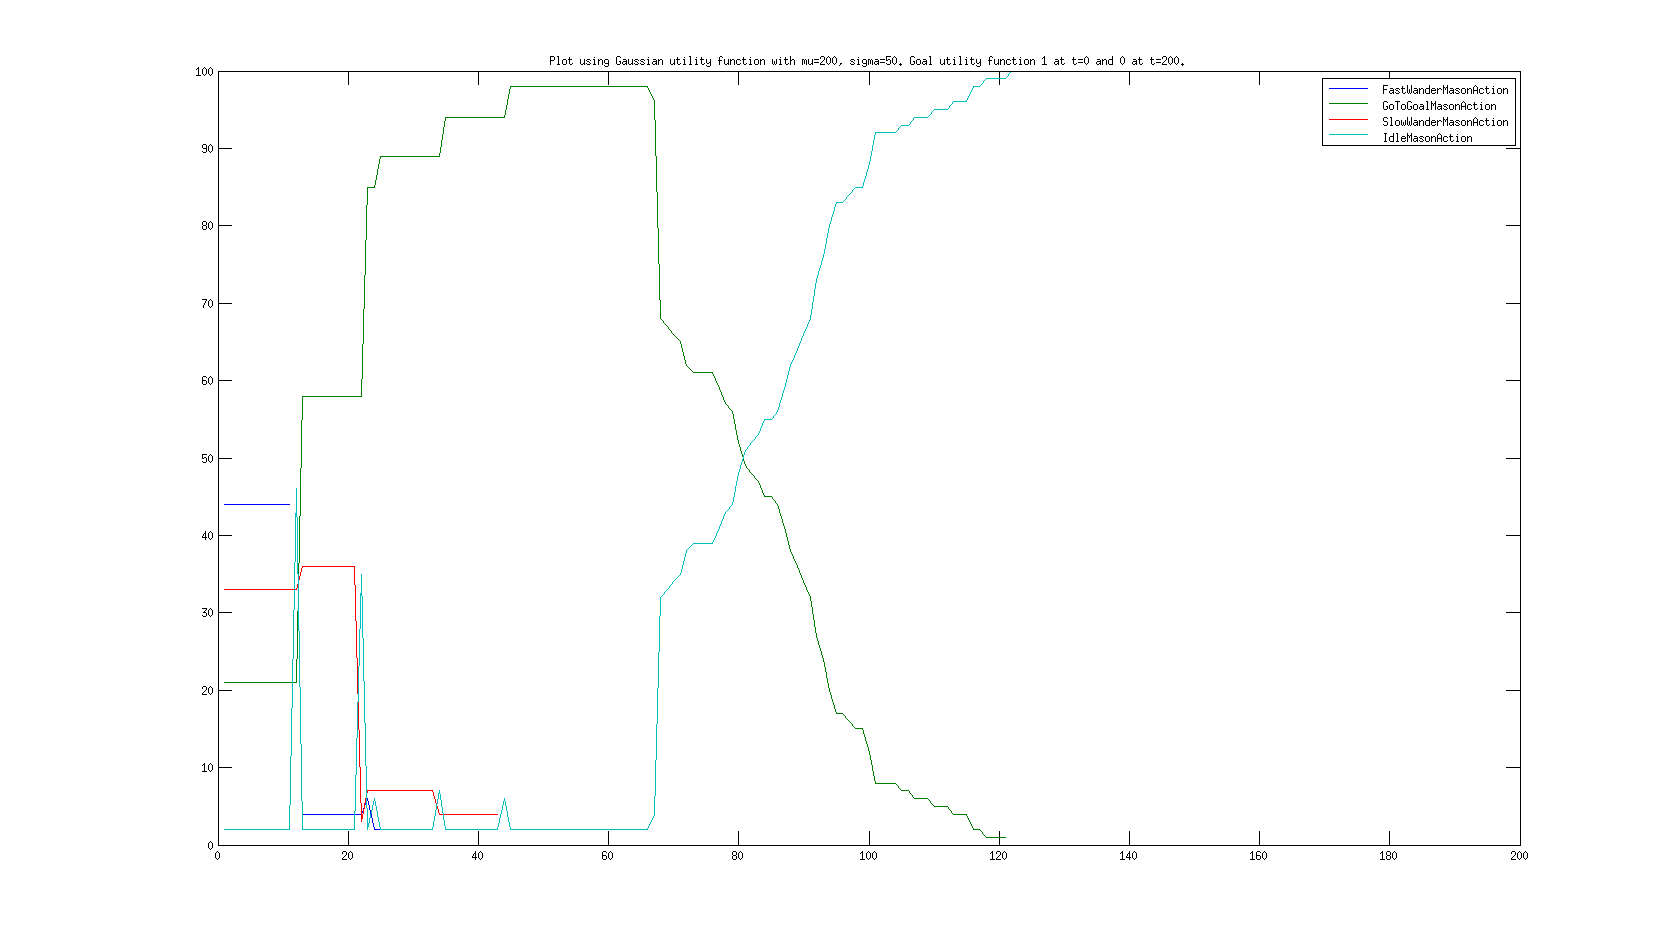
\includegraphics[width=\textwidth]{/home/djura/vakken/svn_afstudeerstage/deadline-driven-behavior/hulpscriptjes/goodresults/gaussian200_50_1_goal1to0.png}
\caption{Goal utility linear with $U_0=1$ and $U_n = 0$. Other behavior utility Gaussian with $\mu=200$ and $\sigma=50$.}
\label{fig:Gaussian200_50_1_goal1to0}
\end{figure}

%%%%%%%%%%%%%%%%%%%%%%%%%%%%%%%%%%%%%%%%%%%%%%%%%%%%%%

In figures \ref{fig:linear0to1_goal01to0}, \ref{fig:sigmoid_100_0_10_1goal01to0} and \ref{fig:gaussian200_50_1_goal01to0} we see the results for the experiments with the goal utility function with $U_0=0.1$ and $U_n=0$. We varied the utility function of the other behavior the same as before. For some reason, the go-to-toilet and wait-for-friend actions are not present in this simulation. They have been replaced by the stand-still action. We would have expected to see more variation in actions now the utility of the go-to-goal behavior has been lowered. Instead, the time-consuming go-to-toilet behavior has been replaced by the less demanding stand-still behavior.

\begin{figure}[h!]
\centering
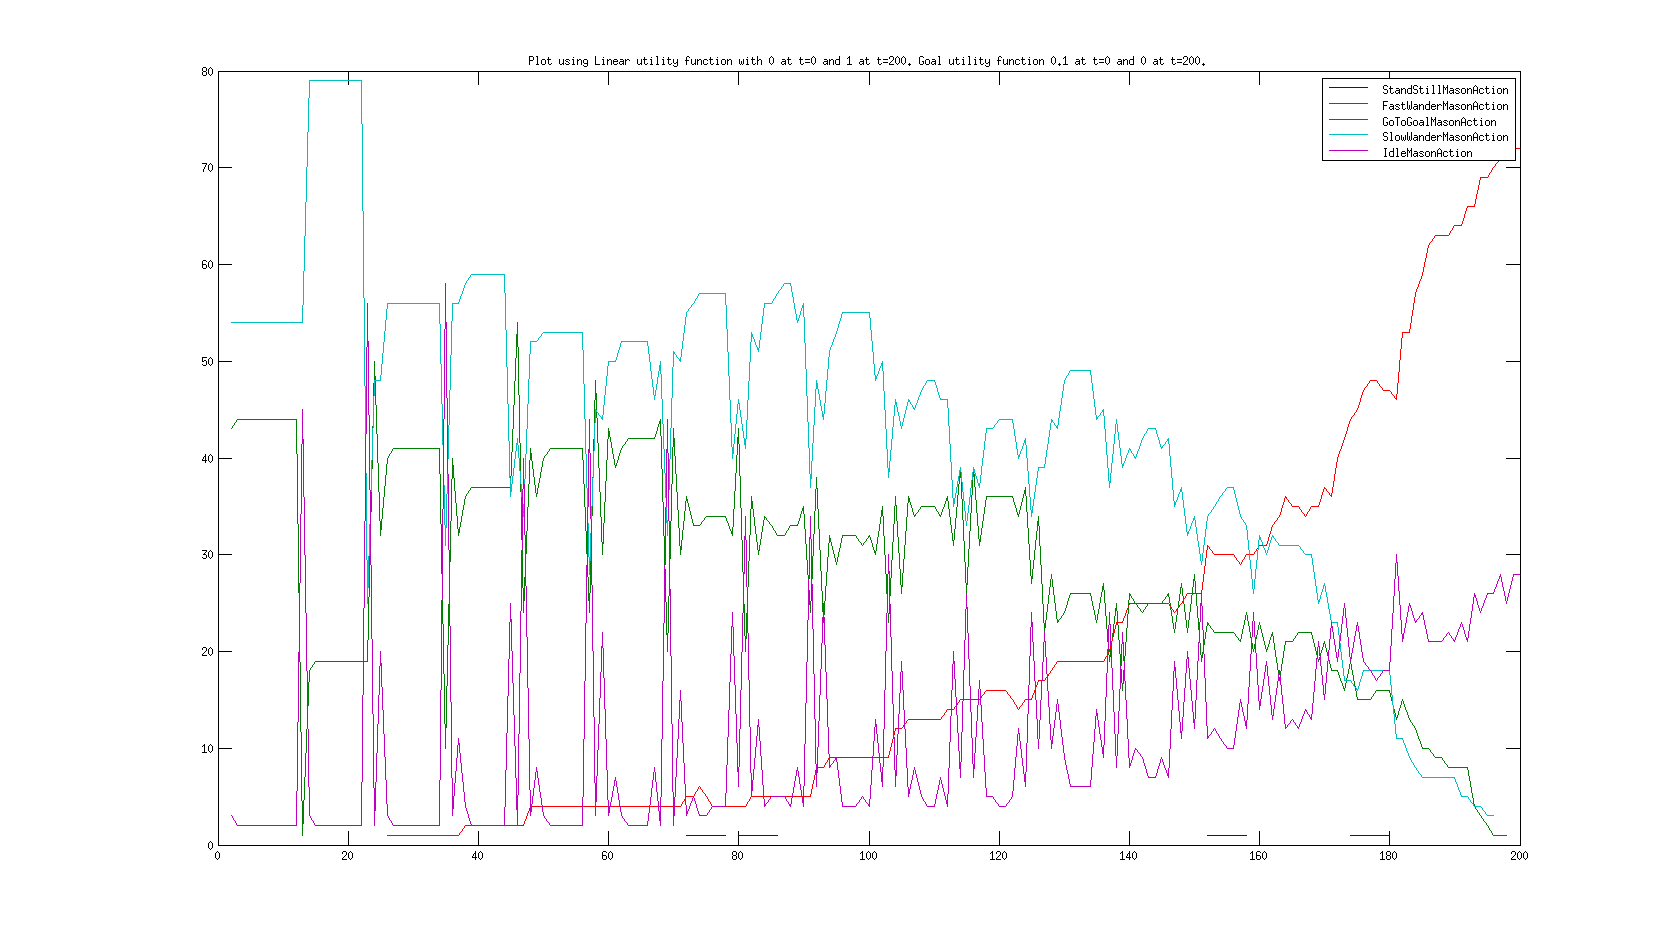
\includegraphics[width=\textwidth]{/home/djura/vakken/svn_afstudeerstage/deadline-driven-behavior/hulpscriptjes/goodresults/linear0to1_goal01to0.png}
\caption{Goal utility linear with $U_0=0.1$ and $U_n=0$. Other utility linear with $U_0=0$ and $U_n=1$}
\label{fig:linear0to1_goal01to0}
\end{figure}

\begin{figure}[h!]
\centering
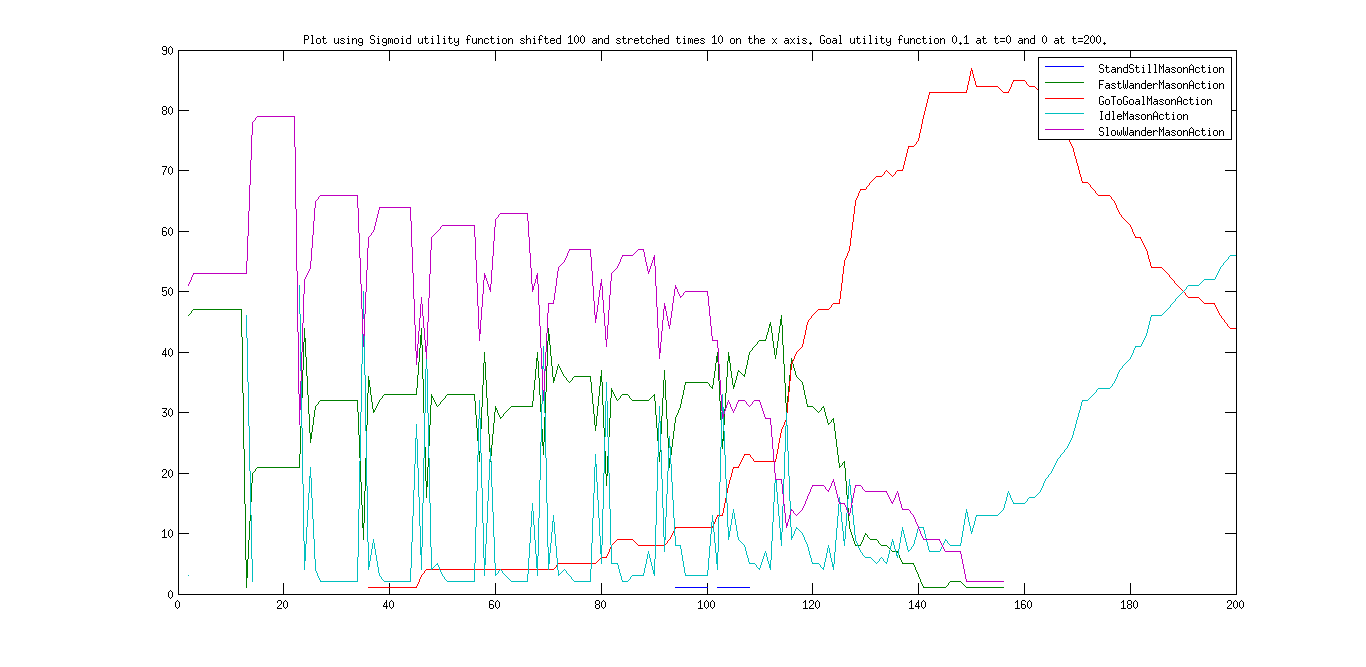
\includegraphics[width=\textwidth]{/home/djura/vakken/svn_afstudeerstage/deadline-driven-behavior/hulpscriptjes/goodresults/sigmoid_100_0_10_1goal01to0.png}
\caption{Goal utility linear with $U_0=0.1$ and $U_n=0$. Other utility sigmoid with $t_0=100$ $\beta=0$ $\omega=10$ $\eta=1$.}
\label{fig:sigmoid_100_0_10_1goal01to0}
\end{figure}

\begin{figure}[h!]
\centering
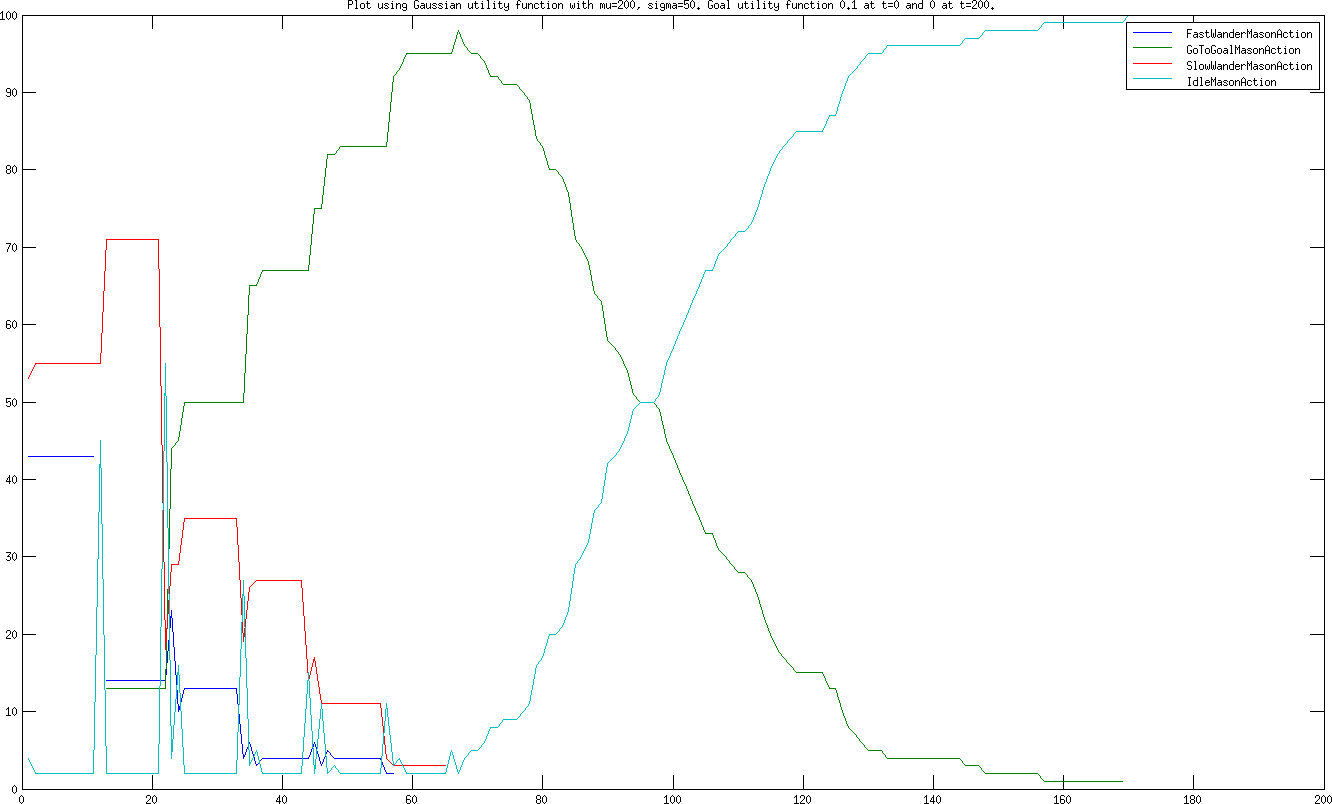
\includegraphics[width=\textwidth]{/home/djura/vakken/svn_afstudeerstage/deadline-driven-behavior/hulpscriptjes/goodresults/gaussian200_50_1_goal01to0.png}
\caption{Goal utility linear with $U_0=0.1$ and $U_n=0$. Other utility Gaussian with $\mu=200$ and $\sigma=50$.}
\label{fig:gaussian200_50_1_goal01to0}
\end{figure}

\clearpage
%%%%%%%%%%%%%%%%%%%%%%%%%%%%%%%%%%%%%%%%%%%%%%%%%%%%%%

In figure \ref{fig:linear0_1_200_goalsigmoid_100_0_-10_1}, \ref{fig:sigmoid100_0_10_1_goalsigmoid100_0_-10_1} and \ref{fig:gaussian200_50_1_goalsigmoid_100_0_-10_1} are the results for the experiments with a sigmoid goal utility function where $t_0=100$, $\beta=1$, $\omega=-10$ and $\eta=1$. The effects are more or less the same as for the previous results. Again, the sigmoid goal utility function causes the pedestrians to go to the goal very soon, eliminating the possibility to do other behavior very soon in the simulation.

\begin{figure}[h!]
\centering
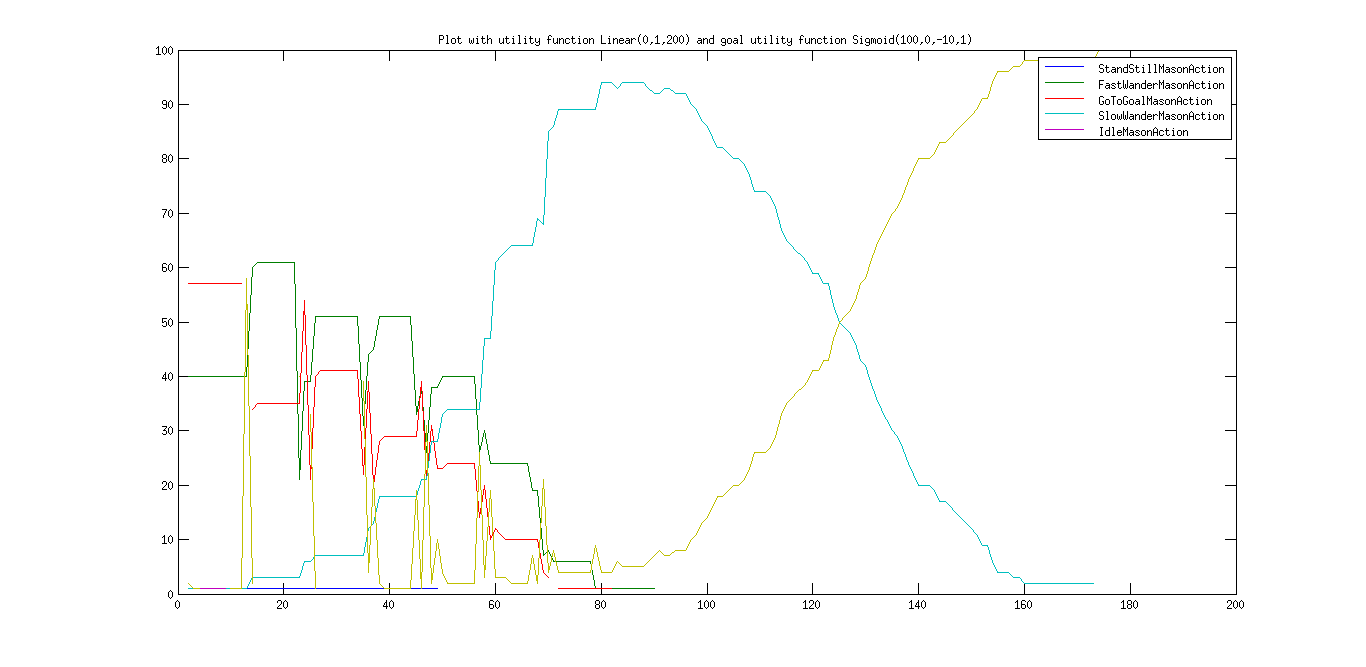
\includegraphics[width=\textwidth]{/home/djura/vakken/svn_afstudeerstage/deadline-driven-behavior/hulpscriptjes/goodresults/linear0_1_200_goalsigmoid_100_0_-10_1.png}
\caption{Goal utility sigmoid with $t_0=100$ $\beta=0$ $\omega=-10$ $\eta=1$. Other utility linear with $U_0=0$ and $U_n=1$}
\label{fig:linear0_1_200_goalsigmoid_100_0_-10_1}
\end{figure}


\begin{figure}[h!]
\centering
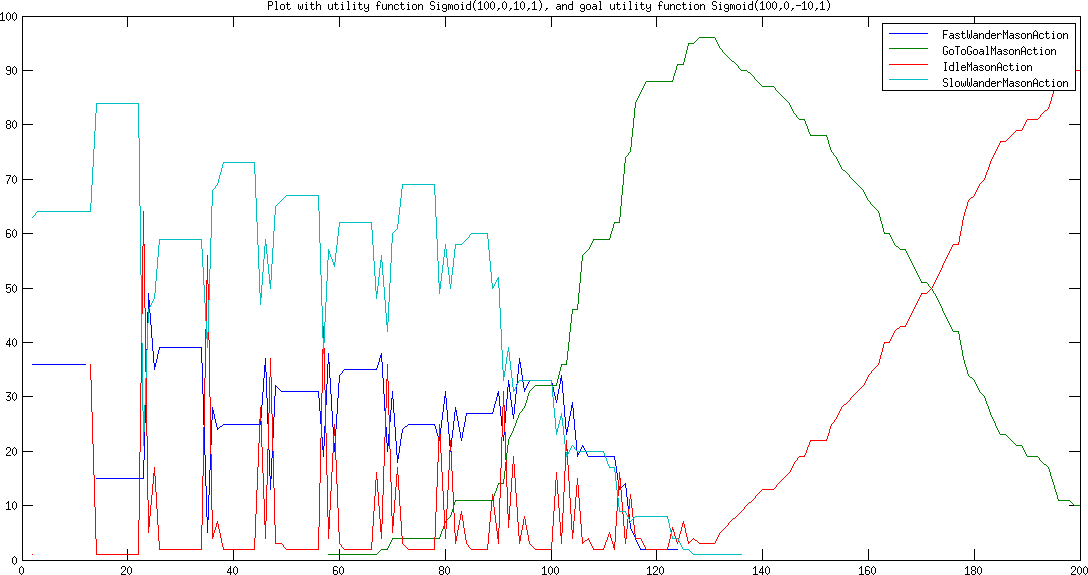
\includegraphics[width=\textwidth]{/home/djura/vakken/svn_afstudeerstage/deadline-driven-behavior/hulpscriptjes/goodresults/sigmoid100_0_10_1_goalsigmoid100_0_-10_1.png}
\caption{Goal utility sigmoid with $t_0=100$ $\beta=0$ $\omega=-10$ $\eta=1$. Other utility sigmoid with $t_0=100$ $\beta=0$ $\omega=10$ $\eta=1$.}
\label{fig:sigmoid100_0_10_1_goalsigmoid100_0_-10_1}
\end{figure}

\begin{figure}[h!]
\centering
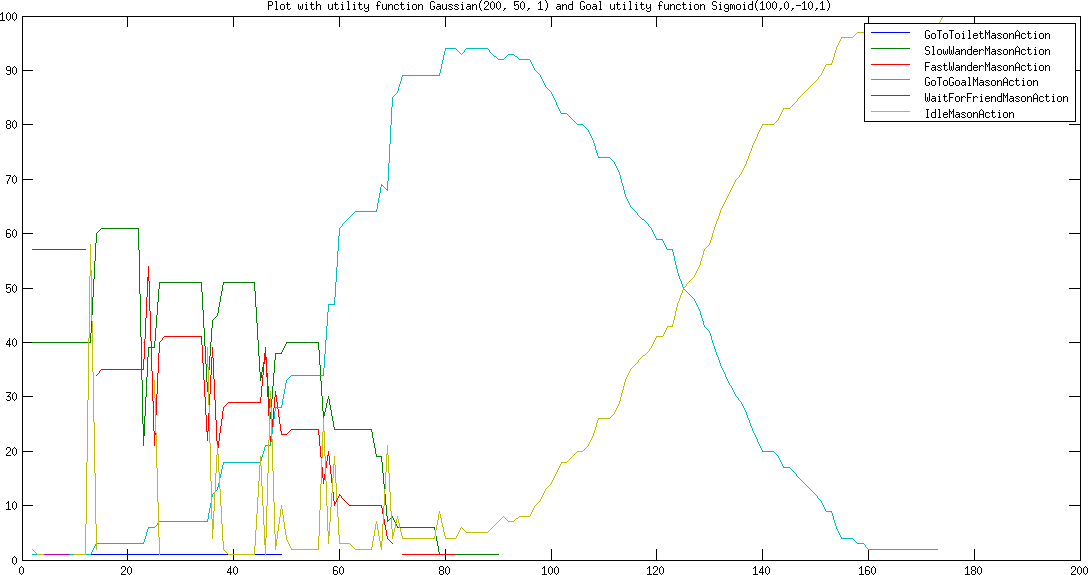
\includegraphics[width=\textwidth]{/home/djura/vakken/svn_afstudeerstage/deadline-driven-behavior/hulpscriptjes/goodresults/gaussian200_50_1_goalsigmoid_100_0_-1_1.png}
\caption{Goal utility sigmoid with $t_0=100$ $\beta=0$ $\omega=-10$ $\eta=1$. Other utility Gaussian with $\mu=200$ and $\sigma=50$.}
\label{fig:gaussian200_50_1_goalsigmoid_100_0_-10_1}
\end{figure}

The results for a Gaussian goal probability function are shown in figure \ref{fig:sigmoid100_0_10_1_goalgaussian0_50_1}, \ref{fig:linear0_1_200_goalgaussian_0_50_1} and \ref{fig:gaussian200_50_1_goalgaussian0_50_1}. We see that in general, the pedestrians seem to wait longer before they go to their goals. This also causes more pedestrians to be too late, because they still are on their way to the goal when the deadline passes. This is very likely due to the fact that the estimation of going to the goal is too low for some pedestrians, because the area they move in is larger than I took into account when estimating the time needed to go to the goal. 

\begin{figure}[h]
\centering
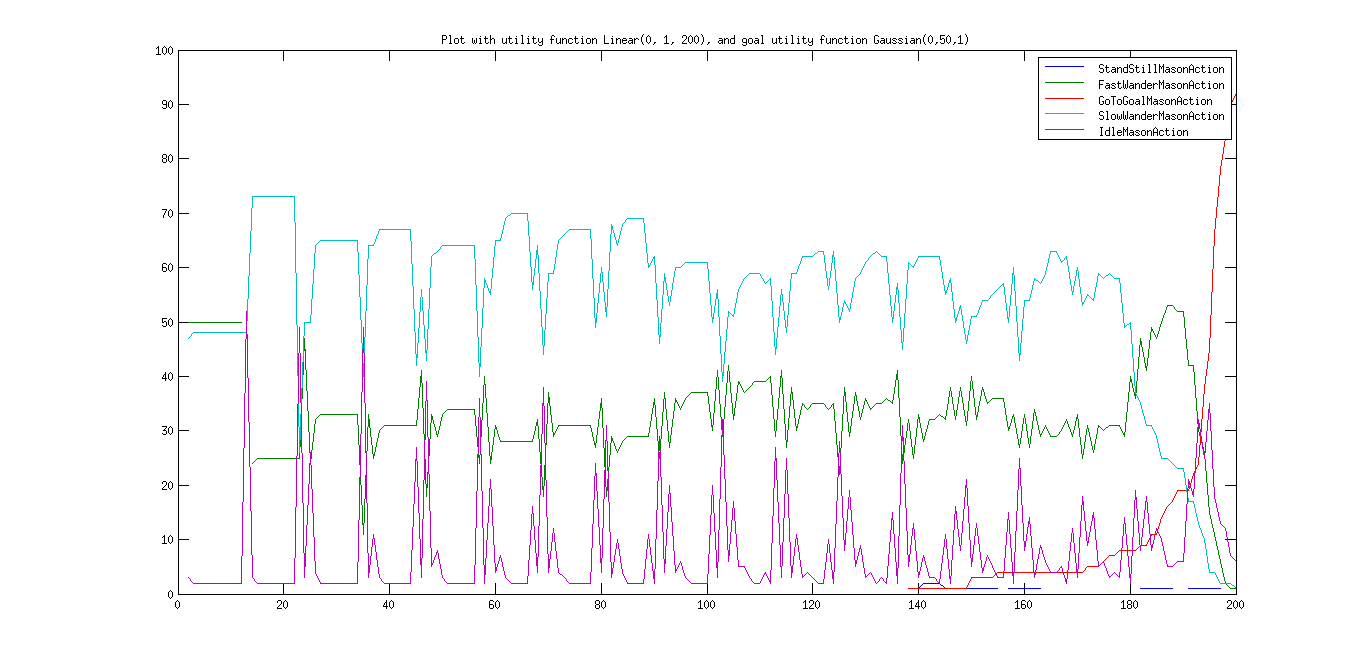
\includegraphics[width=\textwidth]{/home/djura/vakken/svn_afstudeerstage/deadline-driven-behavior/hulpscriptjes/goodresults/linear0_1_200_goalgaussian_0_50_1.png}
\caption{Goal utility Gaussian with $\mu=0$ and $\sigma=50$. Other utility linear with $U_0=0$ and $U_n=1$}
\label{fig:linear0_1_200_goalgaussian_0_50_1}
\end{figure}

\begin{figure}[h]
\centering
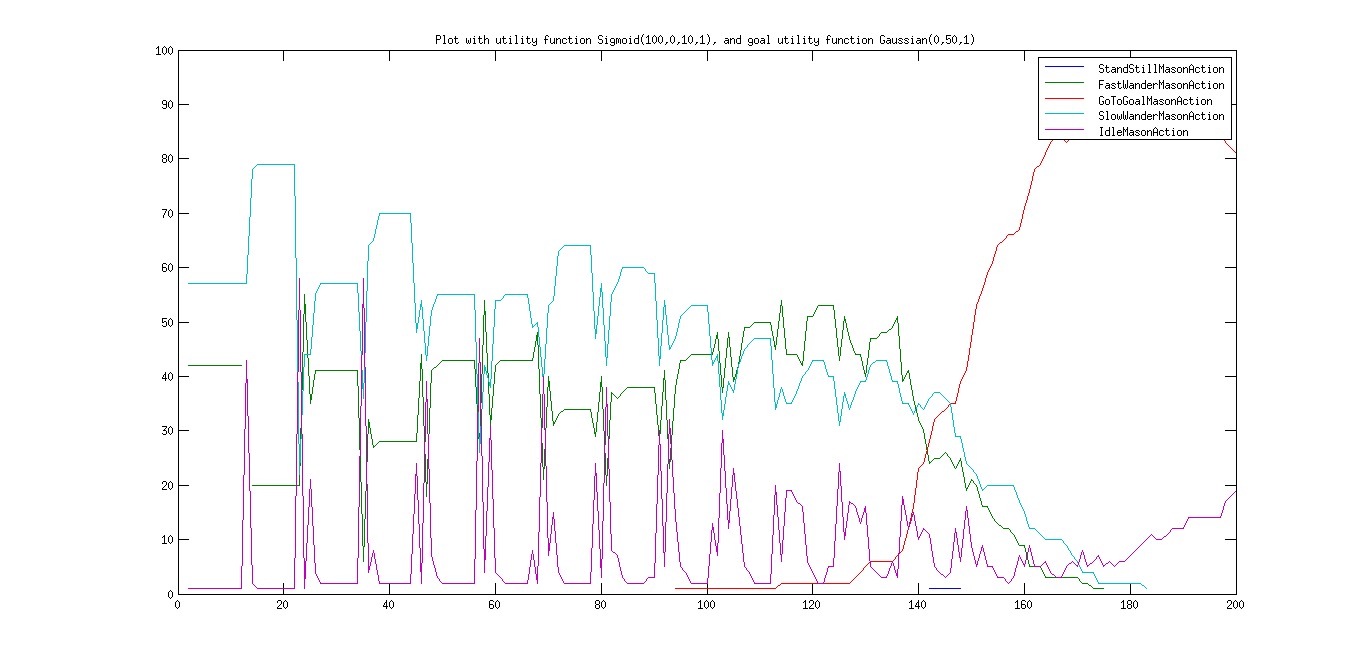
\includegraphics[width=\textwidth]{/home/djura/vakken/svn_afstudeerstage/deadline-driven-behavior/hulpscriptjes/goodresults/sigmoid100_0_10_1_goalgaussian0_50_1.png}
\caption{Goal utility Gaussian with $\mu=0$ and $\sigma=50$. Other utility sigmoid with $t_0=100$ $\beta=0$ $\omega=10$ $\eta=1$.}
\label{fig:sigmoid100_0_10_1_goalgaussian0_50_1}
\end{figure}

\begin{figure}[h]
\centering
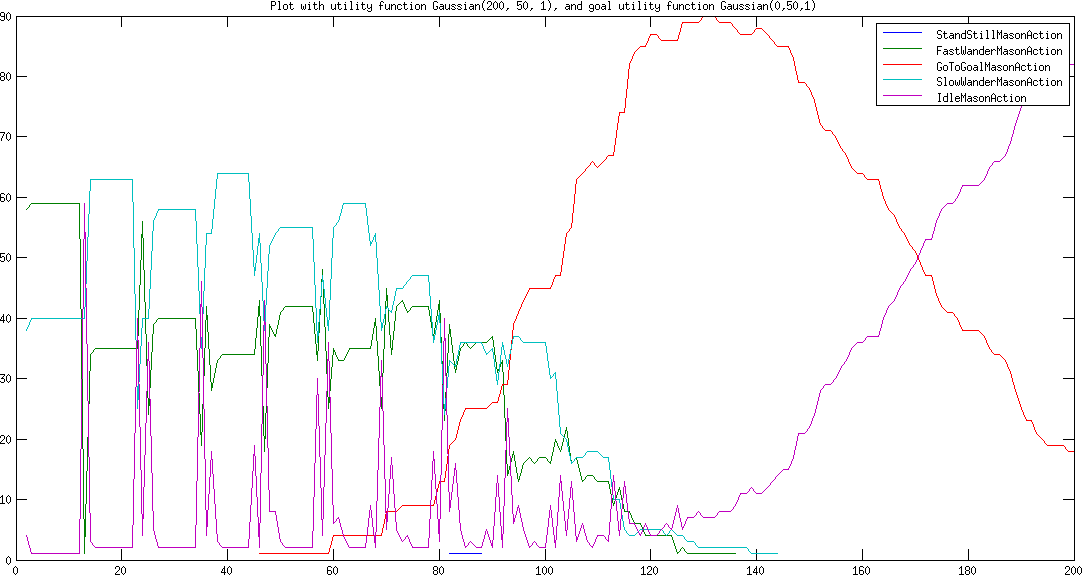
\includegraphics[width=\textwidth]{/home/djura/vakken/svn_afstudeerstage/deadline-driven-behavior/hulpscriptjes/goodresults/gaussian200_50_1_goalgaussian0_50_1.png}
\caption{Goal utility Gaussian with $\mu=0$ and $\sigma=50$. Other utility Gaussian with $\mu=200$ and $\sigma=50$.}
\label{fig:gaussian200_50_1_goalgaussian0_50_1}
\end{figure}
\clearpage

From these results we can make a table in which we judge the utility functions on two important aspects: change from relaxed to hurried behavior (table \ref{tab:judgegoalhurry}) and deadline-drivenness in table \ref{tab:judgegoaldeadline} (do they reach the goal in time?). We give the graphs a score in the following way: when it scores sufficiently, we give an s. If they score better, we have + and ++, and for worse, -- and -- --. We also gave a special score in table \ref{tab:judgegoaldeadline}, namely $>>$. It means that the pedestrians reached their goal too early. When we would judge in terms of whether they are on time, we should have given them ++. However, the pedestrians reached their goal so early that they hardly did any other behavior than going to their goal. This is not desirable, so we decided to score them differently.\\
When looking at the tables, there is only one combination of utility functions that scores sufficiently or better on both categories. A Gaussian goal utility function combined with a sigmoid non-goal utility seems to behave the best in our simulation.

\begin{table}[h!]
\centering
\begin{tabular}{|c|c|c|c|c|c|}
\hline
 & \multicolumn{5}{c|}{Goal}\\
 \hline
 & & Linear & Linear to 0.1 & Sigmoid & Gaussian\\
 \hline
 \multirow{3}{*}{Non-goal} & L & -- & + & -- & s\\
 & S & -- & s & -- & s\\
 & G & -- -- & -- -- & -- -- & --\\
 \hline
\end{tabular}
\caption{Utility functions judged by change from relaxed to hurried behavior}
\label{tab:judgegoalhurry}
\end{table}

\begin{table}[h!]
\centering
\begin{tabular}{|c|c|c|c|c|c|}
\hline
 &  & \multicolumn{4}{c|}{Goal} \\ 
\hline 
 &  & L & L to 0.1 & S & G \\ 
\hline 
\multirow{3}{*}{Non-goal} & L & + & -- -- & s & -- \\ 
 & S & ++ & -- & + & ++ \\ 
 & G & $>>$ & $>>$ & ++ & + \\ 
\hline 
\end{tabular} 
\caption{Utility functions judged by if the pedestrians reach the deadline soon enough.}
\label{tab:judgegoaldeadline}
\end{table}

\todo[inline]{Make table \ref{tab:judgegoalhurry} and \ref{tab:judgegoaldeadline} prettier.}
%\todo[inline]{What should I do with figure \ref{fig:linear0to1goal01}?}
%
%\begin{figure}[h]
%\centering
%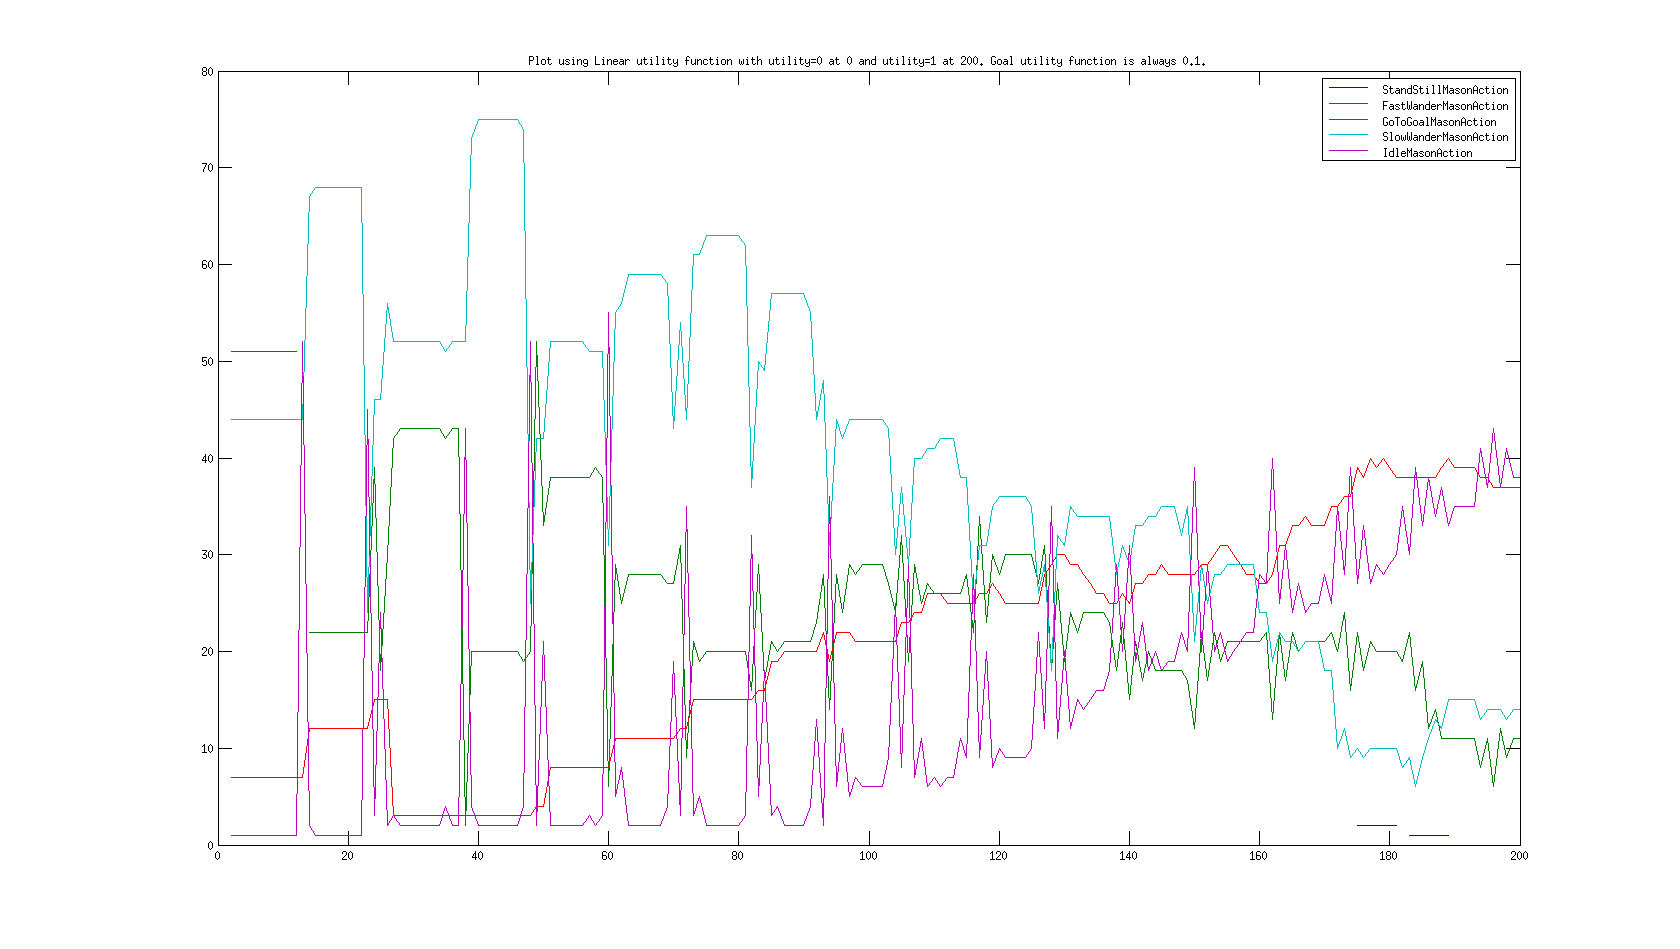
\includegraphics[width=\textwidth]{/home/djura/vakken/svn_afstudeerstage/deadline-driven-behavior/hulpscriptjes/goodresults/linear0to1goal01.png}
%\caption{linear0to1goal01}
%\label{fig:linear0to1goal01}
%\end{figure}


\todo[inline]{Include subsections?}
In short, a number of combinations of utility functions perform well on one of the two criteria, and the combination of a Gaussian goal utility function with a sigmoid non-goal utility performs at least sufficiently on both. We do notice that the goal utility function does start to have a large influence after only a few dozen of steps in most simulations. This way it is possible that the goal utility function "sabotages" the development of a nice transition from hurried to relaxed behavior (we will also talk about this in chapter \ref{chap:conclusiondiscusssion}). This was actually why we decided to do the second quantitative experiment that we described in the previous chapter (\ref{sec:quantitativeexp2}). The results can be found in section \ref{sec:secondquantitativeexperimentresults}.
\todo[inline]{Make sure the utility functions are explained better/clarified. Otherwise it is very confusing that their effect in time is more or less the mirrored version of the way they are defined.}






%%
%%\begin{figure}
%%\centering
%%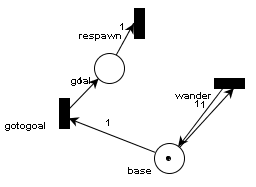
\includegraphics[width=200pt]{rotterdamPedestrianNet}
%%\caption{The basic petrinet for the pedestrian model for Rotterdam airport}
%%\label{basicnet}
%%\end{figure}
%%
%%\begin{figure}
%%\centering
%%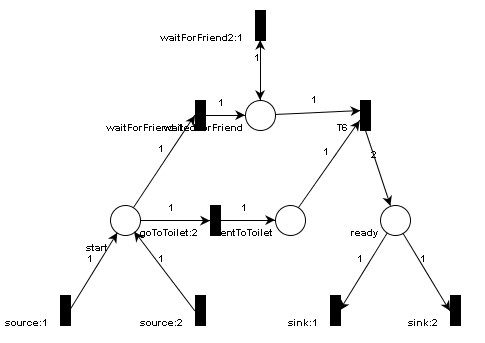
\includegraphics[width=350pt]{twoPeopleToiletSituation}
%%\caption{Behavior model for the toilet situation}
%%\label{toiletsituation}
%%\end{figure}
%%
%%\begin{figure}
%%\centering
%%\includegraphics[width=250pt]{pillarSituation}
%%\caption{Behavior model for the pillar situation}
%%\label{pillarsituation}
%%\end{figure}


\todo[inline]{At this place there was previously a lot of stuff that I now commented out. Decide what to do with it. I shouldn´t put the missing graphs in my thesis in this form. Check if there is still useful stuff in there.}
\clearpage

\section{Results of the Second Quantitative Experiment}
\label{sec:secondquantitativeexperimentresults}
In the first experiment, the go-to-goal behavior was so dominant that it was difficult judge other emergent behavior. The following results will give a clearer view of whether hurried and relaxed behavior can emerge from our framework.

First of all, we have figure \ref{fig:constant1} where the $U=1$ for all $t$. We see the typical phases that we saw in section \ref{sec:firstquantitative} where most pedestrians execute slow- or fast wander for a while, after which the frequency of idle behavior goes up for a few steps. We can also see a few pedestrians doing the go-to-toilet and the accompanying wait-for-friend action. The frequencies of the actions deviate more or less around the same value through the whole simulation.

\begin{figure}
\centering
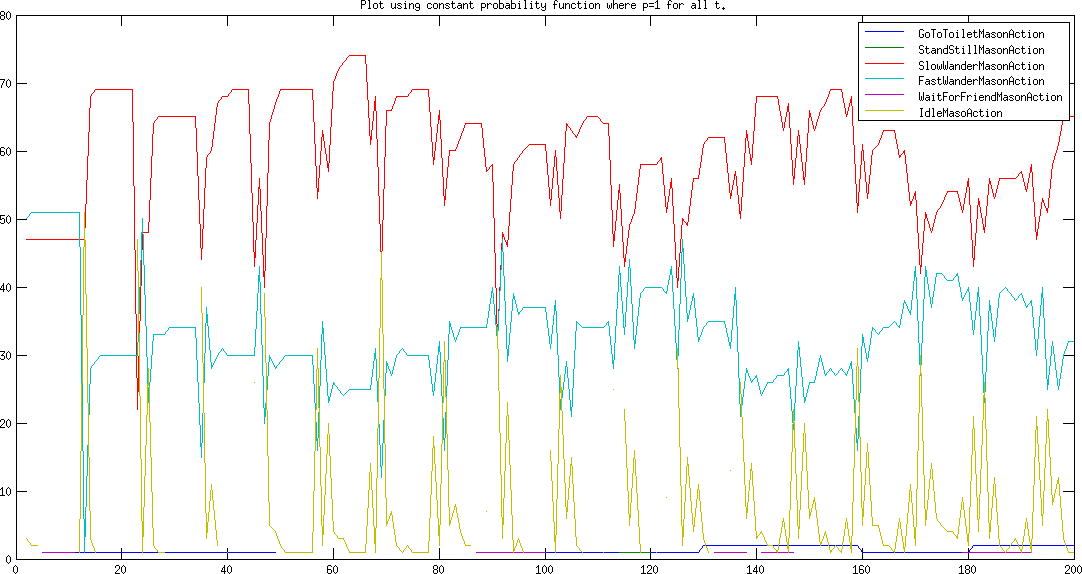
\includegraphics[width=\textwidth]{/home/djura/vakken/svn_afstudeerstage/deadline-driven-behavior/hulpscriptjes/goodresults/constant1_cropped}
\caption{Non goal utility is constant with $U=1$}
\label{fig:constant1}
\end{figure}

Next, we have the results for the utility functions that do decrease when time runs out. It is very clear that eliminating the goal gives the pedestrians the freedom to do different kinds of behavior. We see that the slow wander action has the preference most of the time, except when time has almost run out. Slow wander then decreases while fast wander increases, until even this less time consuming action takes too much time, and the pedestrians become idle. This preference of relaxed behavior (slow wander) until that takes to long to catch a deadline and transitioning to hurried behavior (fast wander) is exactly what we wanted to show with our framework.

We see that using a linear function with a lower maximum value gives the same effect as a linear function that has 1 as highest value (fig \ref{fig:linear0to1_100agents}, \ref{fig:linear0to0.5_100agents} and \ref{fig:linear0to01_100agents}. This is probably because the final probabilities of the transitions to the behaviors are calculated by normalizing the utility functions of all possible behaviors so that their sum is 1.

In figure \ref{fig:sigmoid100_0_10_1} we very clearly the influence of the shape of the sigmoid curve. At around 100 steps the pedestrians exchange their preference of relaxed behavior (slow wander) for hurried behavior (fast wander). With a Gaussian utility function, the resulting graph resembles the results of the linear function again for the first part, but after about 180 steps, it is quite different. We saw that with linear utility functions, the frequency of slow wander would decrease first, followed by fast wander, while idle behavior increases. The Gaussian curve never reaches 0, and the probabilities of executing non-goal behaviors are derived from the relation between the other non-goal behaviors (i.e. the non-goal utilities are normalized). Consequently when the go-to-goal behavior is eliminated, the frequency of non-goal behavior will not decrease with a Gaussian curve.
\todo[inline]{Put \ref{fig:linear0to0.5_100agents} and \ref{fig:linear0to01_100agents} in appendix instead of here. They don't add anything.}

\begin{figure}
\centering
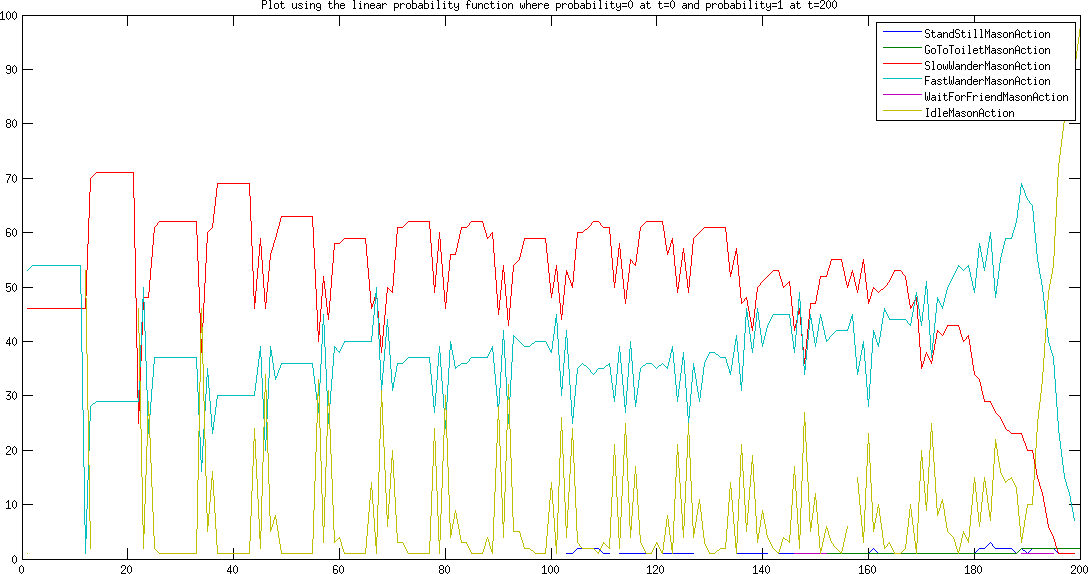
\includegraphics[width=\textwidth]{/home/djura/vakken/svn_afstudeerstage/deadline-driven-behavior/hulpscriptjes/goodresults/linear0to1_100agents.png}
\caption{Non-goal utility linear with $U_0=0$ and $U_n=1$.}
\label{fig:linear0to1_100agents}
\end{figure}


\begin{figure}
\centering
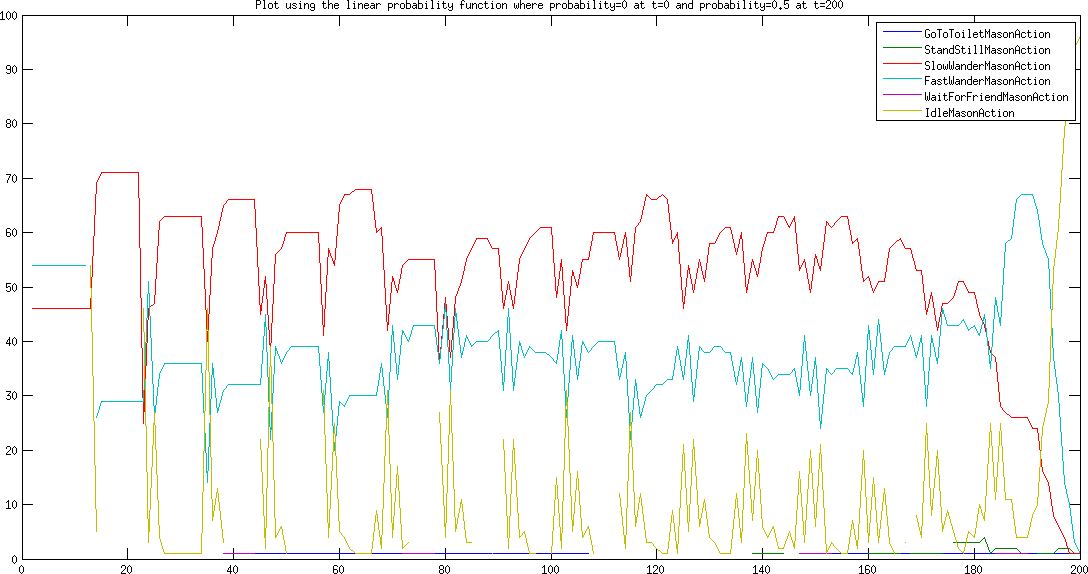
\includegraphics[width=\textwidth]{/home/djura/vakken/svn_afstudeerstage/deadline-driven-behavior/hulpscriptjes/goodresults/linear0to05_100agents.png}
\caption{Non-goal utility linear with $U_0 = 0$ and $U_n=0.5$.}
\label{fig:linear0to0.5_100agents}
\end{figure}

\begin{figure}
\centering
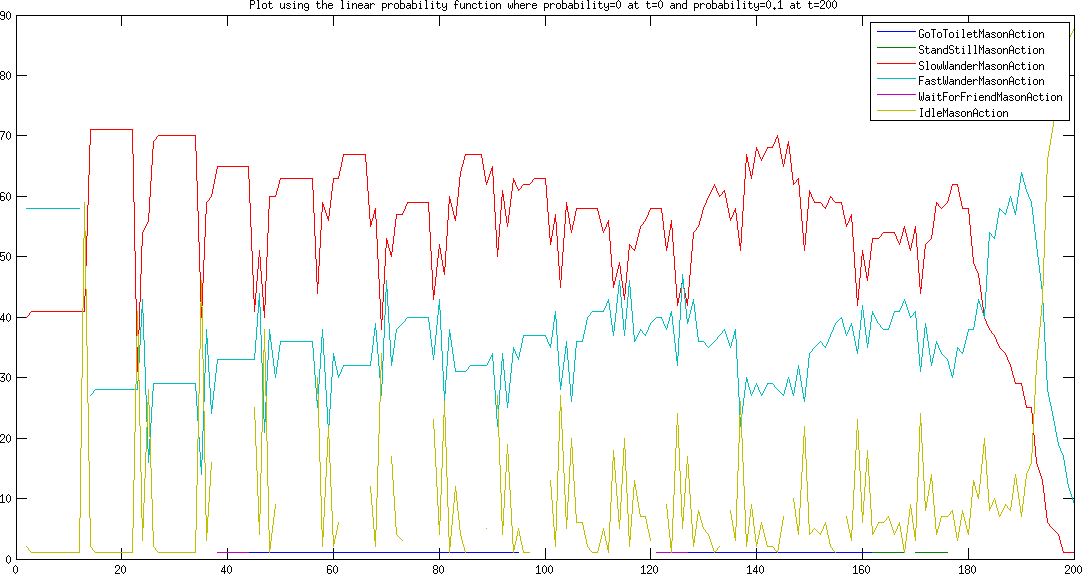
\includegraphics[width=\textwidth]{/home/djura/vakken/svn_afstudeerstage/deadline-driven-behavior/hulpscriptjes/goodresults/linear0to01_100agents.png}
\caption{Non-goal utility linear with $U_0=0$ and $U_n=0.1$.}
\label{fig:linear0to01_100agents}
\end{figure}

\begin{figure}
\centering
\includegraphics[width=\textwidth]{/home/djura/vakken/svn_afstudeerstage/deadline-driven-behavior/hulpscriptjes/goodresults/sigmoid100_0_10_1.png}
\caption{Non-goal utility sigmoid with $t_0=100$ $\beta=0$ $\omega=10$ $\eta=1$.}
\label{fig:sigmoid100_0_10_1}
\end{figure}

\begin{figure}
\centering
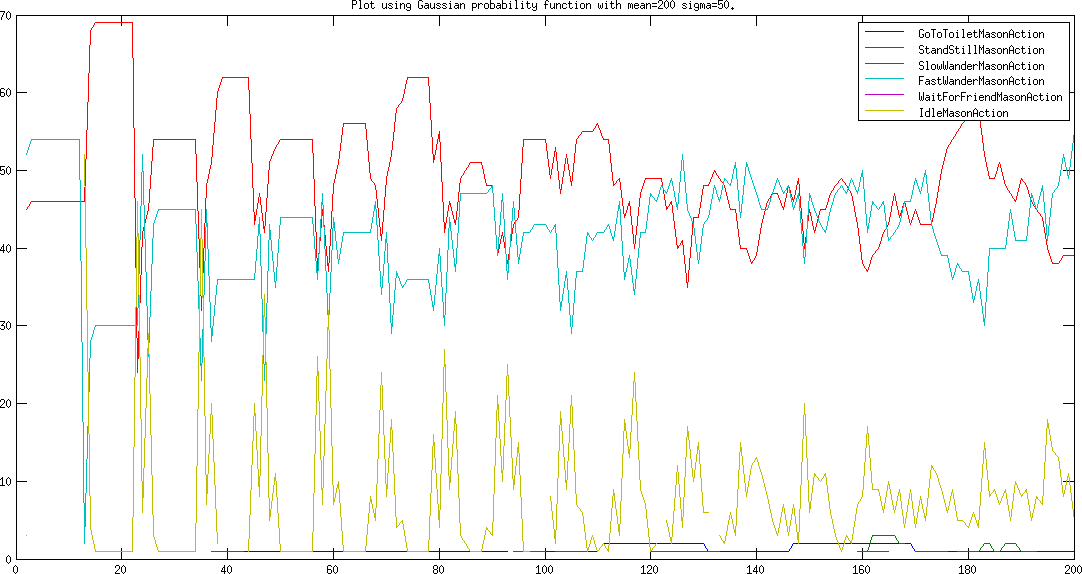
\includegraphics[width=\textwidth]{/home/djura/vakken/svn_afstudeerstage/deadline-driven-behavior/hulpscriptjes/goodresults/gaussian_mean200_sigma50_100_max1.png}
\caption{Non-goal utility Gaussian with $\mu=200$ and $\sigma=50$.}
\label{fig:Gaussian_mean200_sigma50_100_max1}
\end{figure}

We have scored the utility functions again on whether they transition from relaxed to hurried behavior in a realistic manner. The scores can be found in table \ref{tab:secondquantitativetable}. The Gaussian non-goal utility function still results in a poor performance, but with the linear and sigmoid function, the simulation has a better transition from hurried to relaxed behavior than it had when any goal utility function was added.

\begin{table}
\begin{tabular}{|c|c|}
\hline 
 & Relaxed to Hurried\\ 
\hline 
Linear & ++  \\ 
\hline 
Sigmoid & ++  \\ 
\hline 
Gaussian & --\\
\hline
\end{tabular} 
\caption{Scoring table of non-goal utility functions when leaving out go-to-goal action and transition}
\label{tab:secondquantitativetable}
\end{table}

\chapter{Conclusion \& Discussion}
\label{chap:conclusiondiscusssion}
The results are different from what we expected, but logical nonetheless. We expected the sigmoid function to have the ideal curve to reflect the behavior of the pedestrians in Rotterdam airport but
\todo[inline]{Say something about that changing the probabilities of the places is probably only necessary for the sink transitions}


\subsection{Limits of the Deadline Driven Behavior Framework}
Modeling pedestrian behavior with our method does have its limits. First of all, the movements of the agents are designed explicitly through linking together basic movements in the Petri nets. As a consequence, interaction with other agents is quite static, and not directly responsive to surrounding agents. Consequently, our method is not particularly suitable for situations in which the pedestrians have to move very close together, such as when a large amount of pedestrians has to move through a narrow space and have to move closer together or form a queue. When pedestrians move very close together, their behavior will become more uniform, and it would be more sensible to look at the group as a whole, and not as individuals. A more suitable approach would then for example be to look at crowds as particles in a liquid, like Moore, Ali, Mehran and Shah have done \cite{Moore:2011:VCS:2043174.2043192}. Their supposition is that people in crowds seem to move according to the flow, just like particles in a liquid.
\todo[inline]{Integrate the text below and make it better}
Our framework is focused on deciding if a behavior will leave enough time to do the goal behavior before the deadline. Because of the way we did this behaviors that don't take long will always have a slight preference over behavior that take a larger amount of time. There are cases in which this approach does not result in realistic behavior. For example, when a pedestrian has so much time to reach the deadline that even the "relaxed" behavior is possible many times in succession without missing the deadline, people in real life will probably have a large preference for many of the time consuming behavior over the quicker behavior. For example, people will prefer walking slow greatly over running. This preference of slow behavior over fast behavior cannot be implemented in our system as such.

\subsection{Optimization}
It is very well possible that the results found in our research are far from the optimal results we could have gotten with our framework.  Machine learning could be used to attain the optimal deadline driven behavior. However, this is beyond the scope of our research.

\subsection{Future Work}
There are several ways in which the deadline driven behavior framework can be extended. For example, currently, the probabilities for entering situations are only dependent on how close the agent is to the deadline. So, no matter what time of day it is, the pedestrians will always have the same probability to do a certain action. However, in real life, a person's probabilities for certain behavior is also largely dependent on their daily cycle.

\subsubsection{Finding the optimal parameters}

\subsubsection{Needs}
Ideally, a pedestrian's propensity to execute certain actions, such as eating, should vary dependent on whether the individual has recently executed that action, and their daily cycle. In other words, we would like to introduce \emph{needs} to the framework. By introducing the concept of needs, we would be better able to model the daily flow of people in a typical public area. We can vary the needs according to the time of day and whether this need has been fulfilled recently.

\appendix

\chapter{Appendix A: Implementation}
In the appendix we will go into some of the details of implementation of the deadline driven behavior framework. We will also give some directions about how to use our implementation to simulate your own scenario, or to extend it yourself.


\section{Implementing the Framework}


\section{Extending PIPE2}

\subsection{Sources, Sinks, Slots}
In order to facilitate transporting tokens between Petri nets, we created classes of transitions with added functionality to keep track of how these nets are connected. These transitions are called \emph{sinks} and \emph{sources}. A source is a transition that has no incoming connections, only outgoing, with the result that this kind of transition produces new tokens without consuming any, increasing the total amount of tokens in the Petri net. A sink is exactly the opposite: it only consumes tokens and does not produce, effectively decreasing the amount of tokens in the network. Subsequently, we can use these special classes of transitions to transport tokens from one net to another. In order to keep track of how the nets are connected, we pair a sink with every source transition. These pairs are put together in a class called \emph{Slot}.

\subsection{Additional Modifications}


\section{MASON}

\section{Connecting MASON and the Situations Framework}
We deliberately divided our framework into two main modules. Because the situations framework has been implemented with the prospect of interfacing it with other simulations we decided to have the two main units communicate through socket connections. We have the situations side keep track of a thread pool. Every time a pedestrian from the MASON side connects to the situations side, a check is done whether this MASON pedestrian has connected to the Situations before. If this is not the case, another thread will be created to handle the connection to this new pedestrian.  Figure \ref{framework}  shows the global structure. Here you can see how the two interact.
\todo[inline]{Finish this part about MASON}
\begin{itemize}
\item Blabla thread pool
\item blabla 1 kant is niet multithreaded maar whatever
\item ...
\end{itemize}


\chapter{Appendix B: Results}
\begin{figure}
\centering
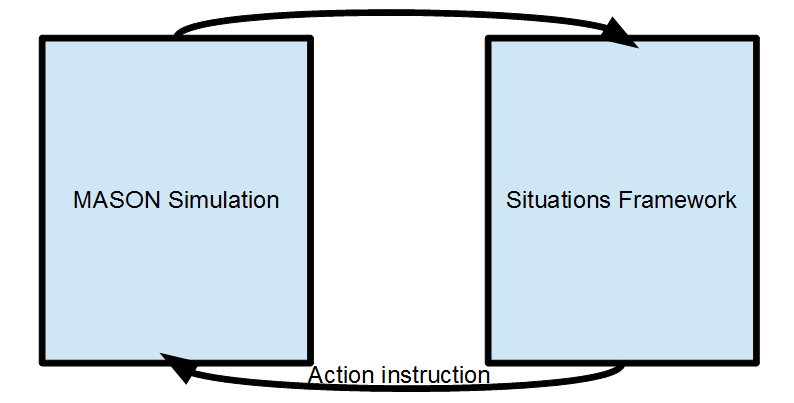
\includegraphics[width=250pt]{framework}
\caption{The global workings of our framework}
\label{framework}
\end{figure}



\bibliographystyle{plain}
\bibliography{references}

\todo[inline]{Check all references (figures, papers, etc.)}

\end{document}
